
% Este documento LaTeX fue diseñado por profesores  del Departamento de Matemáticas 
% de la Universidad de Antioqua (http://ciencias.udea.edu.co/). Usted puede modificarlo
% y personalizarlo a su gusto bajo los términos de la licencia de documentación libre GNU.
% http://es.wikipedia.org/w/index.php?title=Licencia_de_documentaci%C3%B3n_libre_de_GNU&oldid=15717448

\documentclass[serif,9pt, t]{beamer}
\setbeamertemplate{navigation symbols}{}
\addtobeamertemplate{navigation symbols}{}{
    \insertframenumber/\inserttotalframenumber
}
\setbeamercolor{navigation symbols}{fg=black}
\usetheme{Warsaw}

\usepackage[utf8]{inputenc}
\usepackage[spanish]{babel}
\usepackage{verbatim} %para comentarios multilinea
\usepackage{subfig}
\newcommand{\insm}{%
\smash{\raisebox{.5\dimexpr3\baselineskip+4\itemsep+2\parskip}{$\left.\rule{0pt}{.5\dimexpr4\baselineskip+3\itemsep+3\parskip}\right\}$\ \parbox{5.5cm}{Newton Cotes formulae of different degrees}}}
}
\graphicspath{{figuras/}}

\newif\ifplacelogo % Para que el logo solo figure en el primer slide
\placelogotrue
\logo{\ifplacelogo
\includegraphics[scale=0.25]{logo_exactas}\fi}
\newcommand\Fontvi{\fontsize{7}{7.2}\selectfont}

\beamersetuncovermixins{\opaqueness<1>{25}}{\opaqueness<2->{15}}

\begin{document}
\title[Análisis y Detección de Correlaciones en Relevamien\ldots ]{Análisis y Detección de Correlaciones en Relevamientos Transcripcionales de Gran Escala}  
\author[Andrés Rabinovich]{Andrés Rabinovich\\{\small Director: Dr. Ariel Chernomoretz}}

\institute[Departamento de Física]{
	Departamento de Física\\	
	Facultad de Ciencias Exactas y Naturales\\
	Universidad de Buenos Aires}
\date{Marzo 2016.}


\begin{frame}
\titlepage
\end{frame}

\placelogofalse

\begin{frame}\frametitle{Contenido}
\tableofcontents
\end{frame} 

\section{Introducción} 


\subsection{Relevamientos transcripcionales de gran escala}

\subsubsection*{Transcripción y traducción}
\begin{frame}\frametitle{Transcripción y traducción (dogma central de la biología molecular)}
\centering 
Células, ADN, ARNm, proteínas y otras yerbas...
\begin{figure}[t]
  \centering
  \subfloat[Célula eucariota]{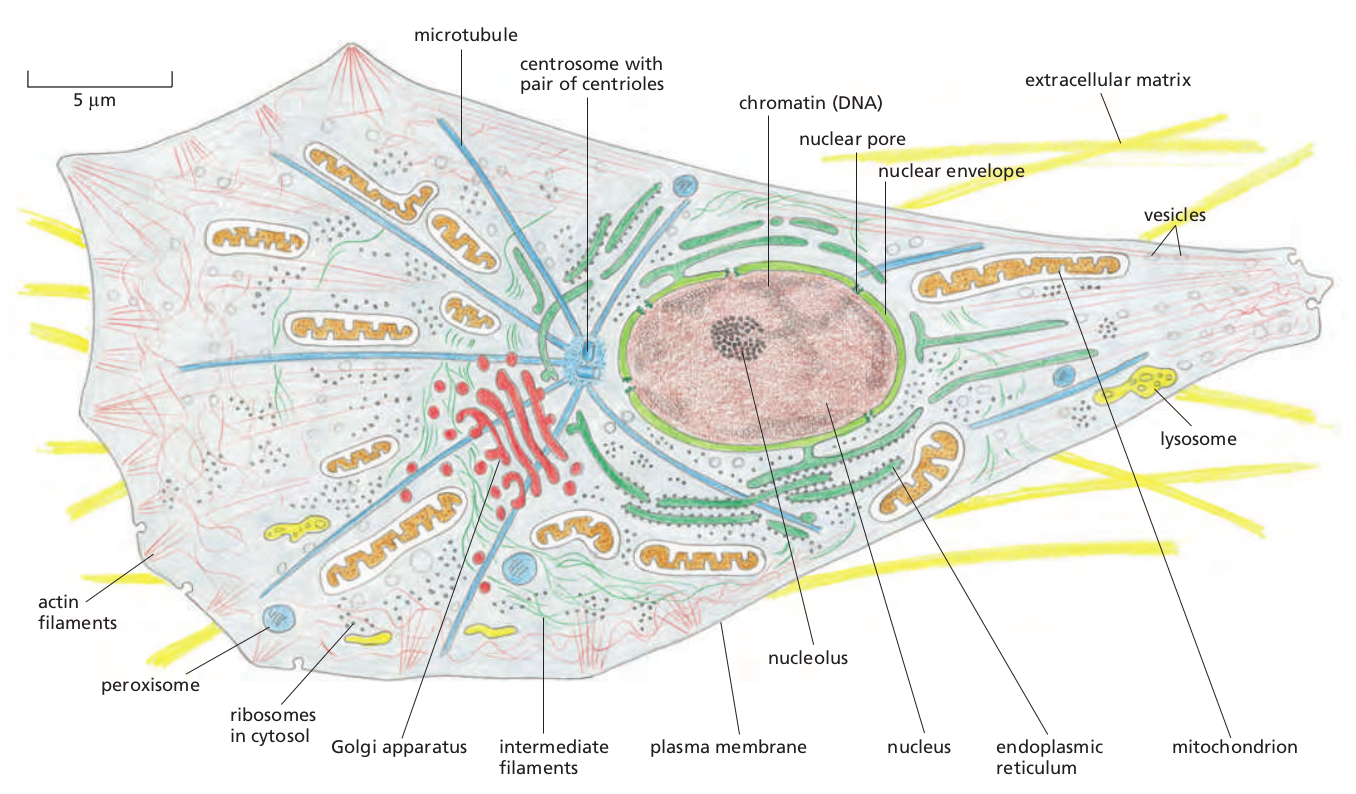
\includegraphics[width=0.5\textwidth]{celula_eucariota}}
  \subfloat[Dogma central de la biología molecular]{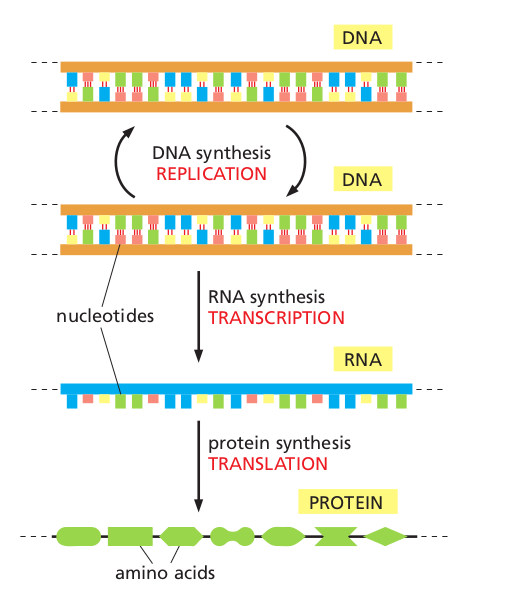
\includegraphics[width=0.5\textwidth]{adn3}}
\end{figure}

\end{frame}

\subsubsection*{Cambios transcripcionales}
\begin{frame}\frametitle{Cambios transcripcionales en respuesta a estrés abiótico en \textit{A. thaliana}} 
	\begin{columns}[T]
		\column{0.5\textwidth}
			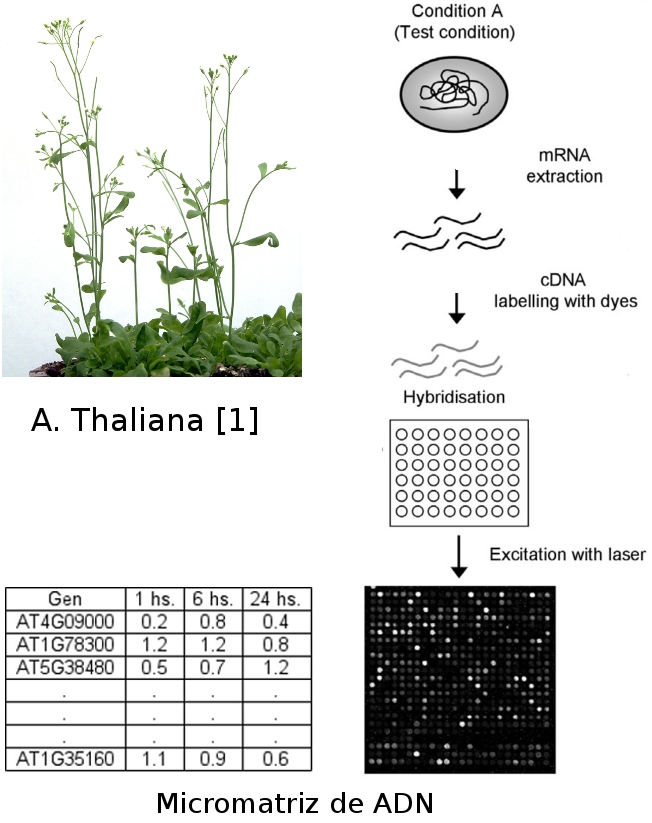
\includegraphics[width=1\textwidth]{micromatriz_y_arabidopsis}
		\column{0.5\textwidth}
			\bigskip
			\Large 
			Datos de estrés abiótico:
			\medskip
			\Fontvi
			\begin{itemize}
				\item 11 tratamientos: frío, calor, osmótico, salinidad, sequía, genotoxicidad, oxidación, UV, herida, recuperación y control.
				\item $\approx 22000$ genes.
				\item Nos quedaremos con un subconjunto de $\approx 6000$ genes que son los que se movieron en algún tratamiento.
				\item entre 4 y 8 mediciones temporales por gen y por tratamiento.
			\end{itemize}			
			\centering	
			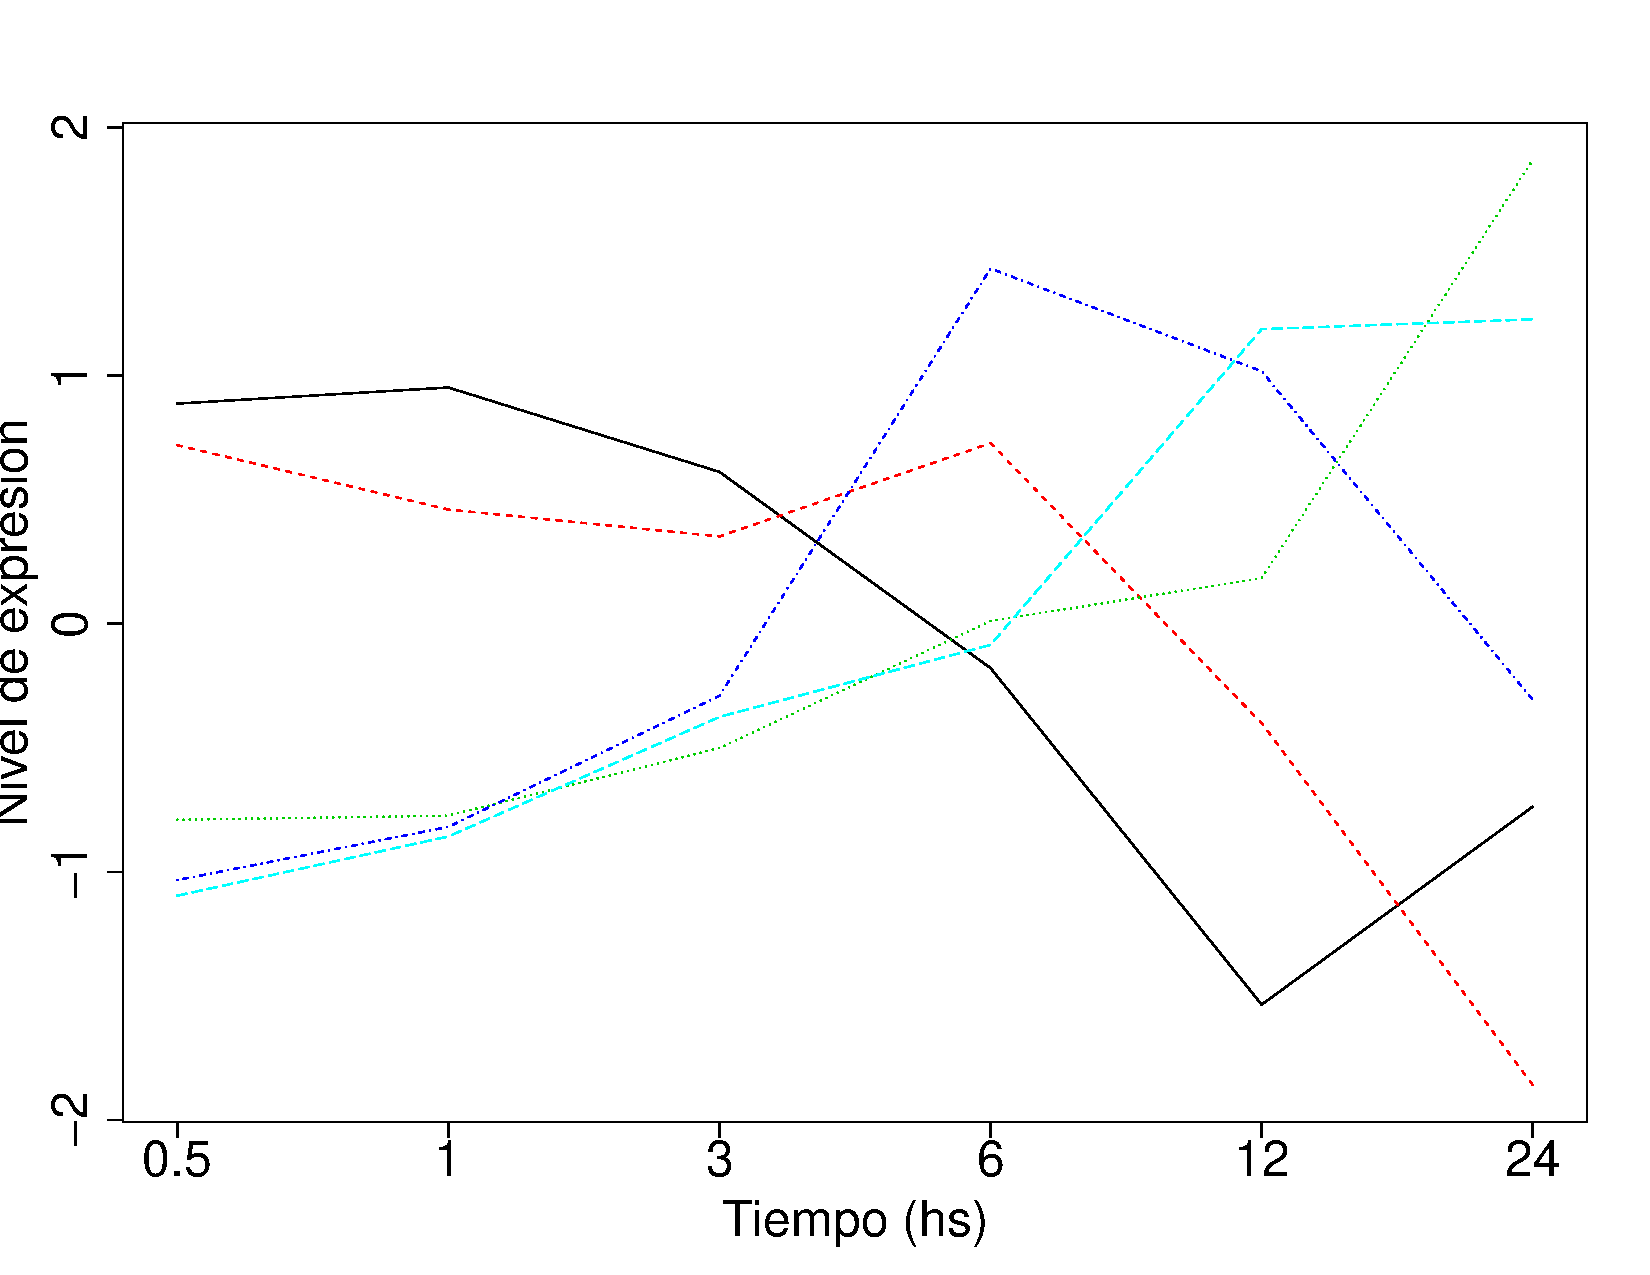
\includegraphics[width=0.7\textwidth]{perfiles_sin_agrupar.pdf}			
	\end{columns}
\end{frame}

\subsection{Detección de correlaciones}
\begin{frame}\frametitle{Detección de correlaciones} 
\large
Queremos inferir estrategias del organismo frente a los tratamientos.\\\bigskip
Lo vamos a hacer usando métodos de agrupamiento o ``clustering'' para encontrar relaciones y estructura en esta gran cantidad de datos.\medskip
\normalsize
\begin{itemize}
\item Son métodos no supervisados.
\item Consisten en agrupar elementos ``similares entre si''.
\item Permiten el descubrimiento de patrones en los datos.
\item Posibilitan obtener conclusiones sobre los datos.
\end{itemize}
\bigskip
\begin{columns}[T]
	\column{0.5\textwidth}
		\Fontvi
		\underline{A modo de ejemplo}\medskip

		El conjunto: $\{-5, -3, -2, 2, 3\}$\medskip

		Agrupado por módulo: $\{-5\}$, $\{-3, 3\}$ y $\{-2, 2\}$\medskip

		Agrupado por signo: $\{-5, -3, -2\}$ y $\{2, 3\}$
	\column{0.5\textwidth}
	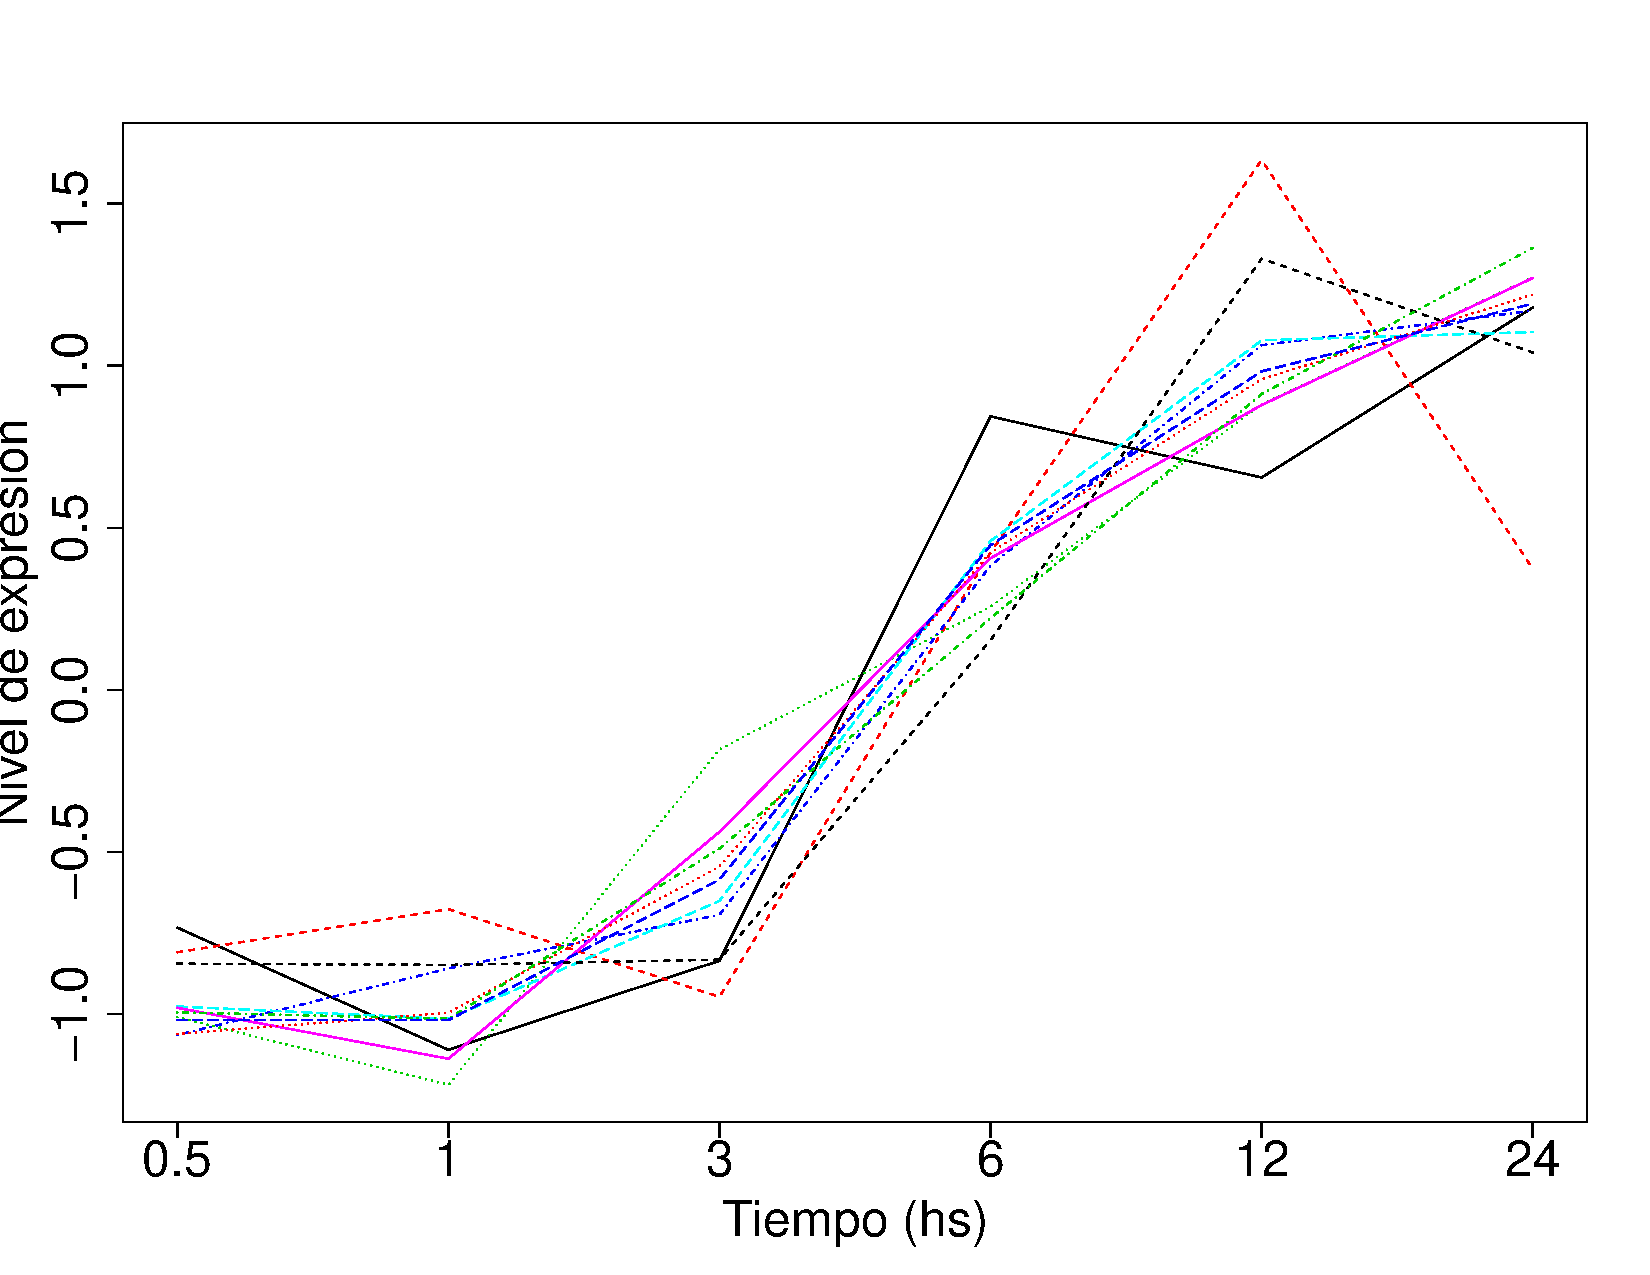
\includegraphics[width=0.8\textwidth]{perfiles_coregulados.pdf}
\end{columns}
\end{frame}

\section{Análisis de relevamientos transcripcionales}

\subsection{Medidas de similaridad y distancia}
\begin{frame} \frametitle{Medidas de similaridad y distancia} 
\centering
	Distancia basada en el coeficiente de correlación de Pearson:\\
	\begin{equation}
		r(\vec{x}, \vec{y}) = \frac{\frac{1}{n-1}\sum\limits_{i=1}^n(x_i-\bar{x})(y_i-\bar{y})}{s_x s_y}
	\end{equation}
	\begin{equation}
		d_{ccp}(\vec{x}, \vec{y}) = 1-r(\vec{x}, \vec{y})
	\end{equation}

	\centering	
	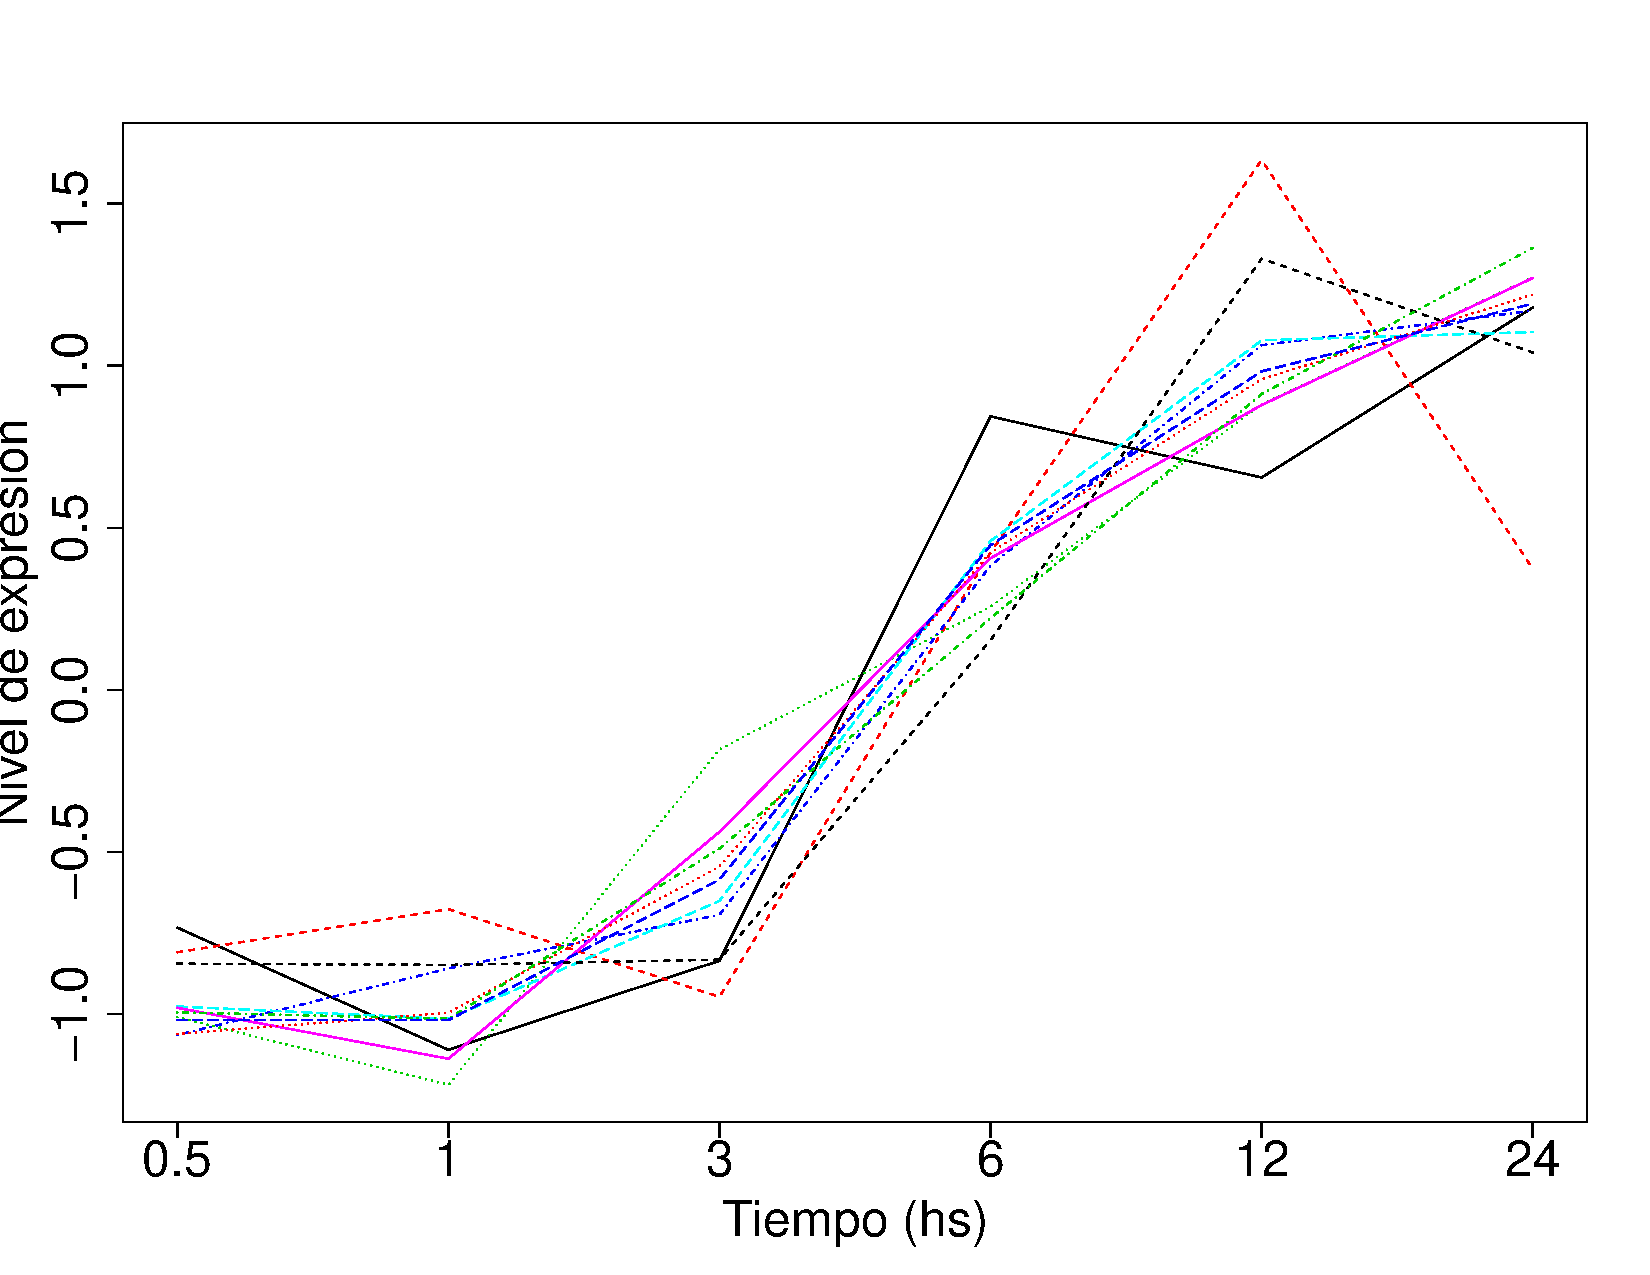
\includegraphics[width=0.45\textwidth]{perfiles_coregulados.pdf}

\end{frame}

\subsection{Métodos de agrupamiento utilizados}
%\begin{frame}\frametitle{Método de agrupamiento k-means} 
%\begin{columns}[T]
%\column{0.5\textwidth}
%	\begin{itemize}
%	\item Agrupamiento no jerárquico.
%	\item Cada observación pertenece al grupo con la media más cercana.
%	\item La cantidad k de grupos debe ser fijada a priori.
%	\item Utiliza la distancia euclidiana.
%	\end{itemize}
%	Para datos estandarizados:
%	\begin{equation}
%		\tilde{x_i} = \frac{x_i-\bar{x}}{s_x}
%	\end{equation}	
%	la distancia euclidiana se relaciona con la correlación como:
%	\begin{equation}
%		d(\vec{x}, \vec{y}) = \sqrt{2(n-1)(1-r(\vec{x}, \vec{y}))}
%	\end{equation}

%\column{0.5\textwidth}
%	\centering	
%	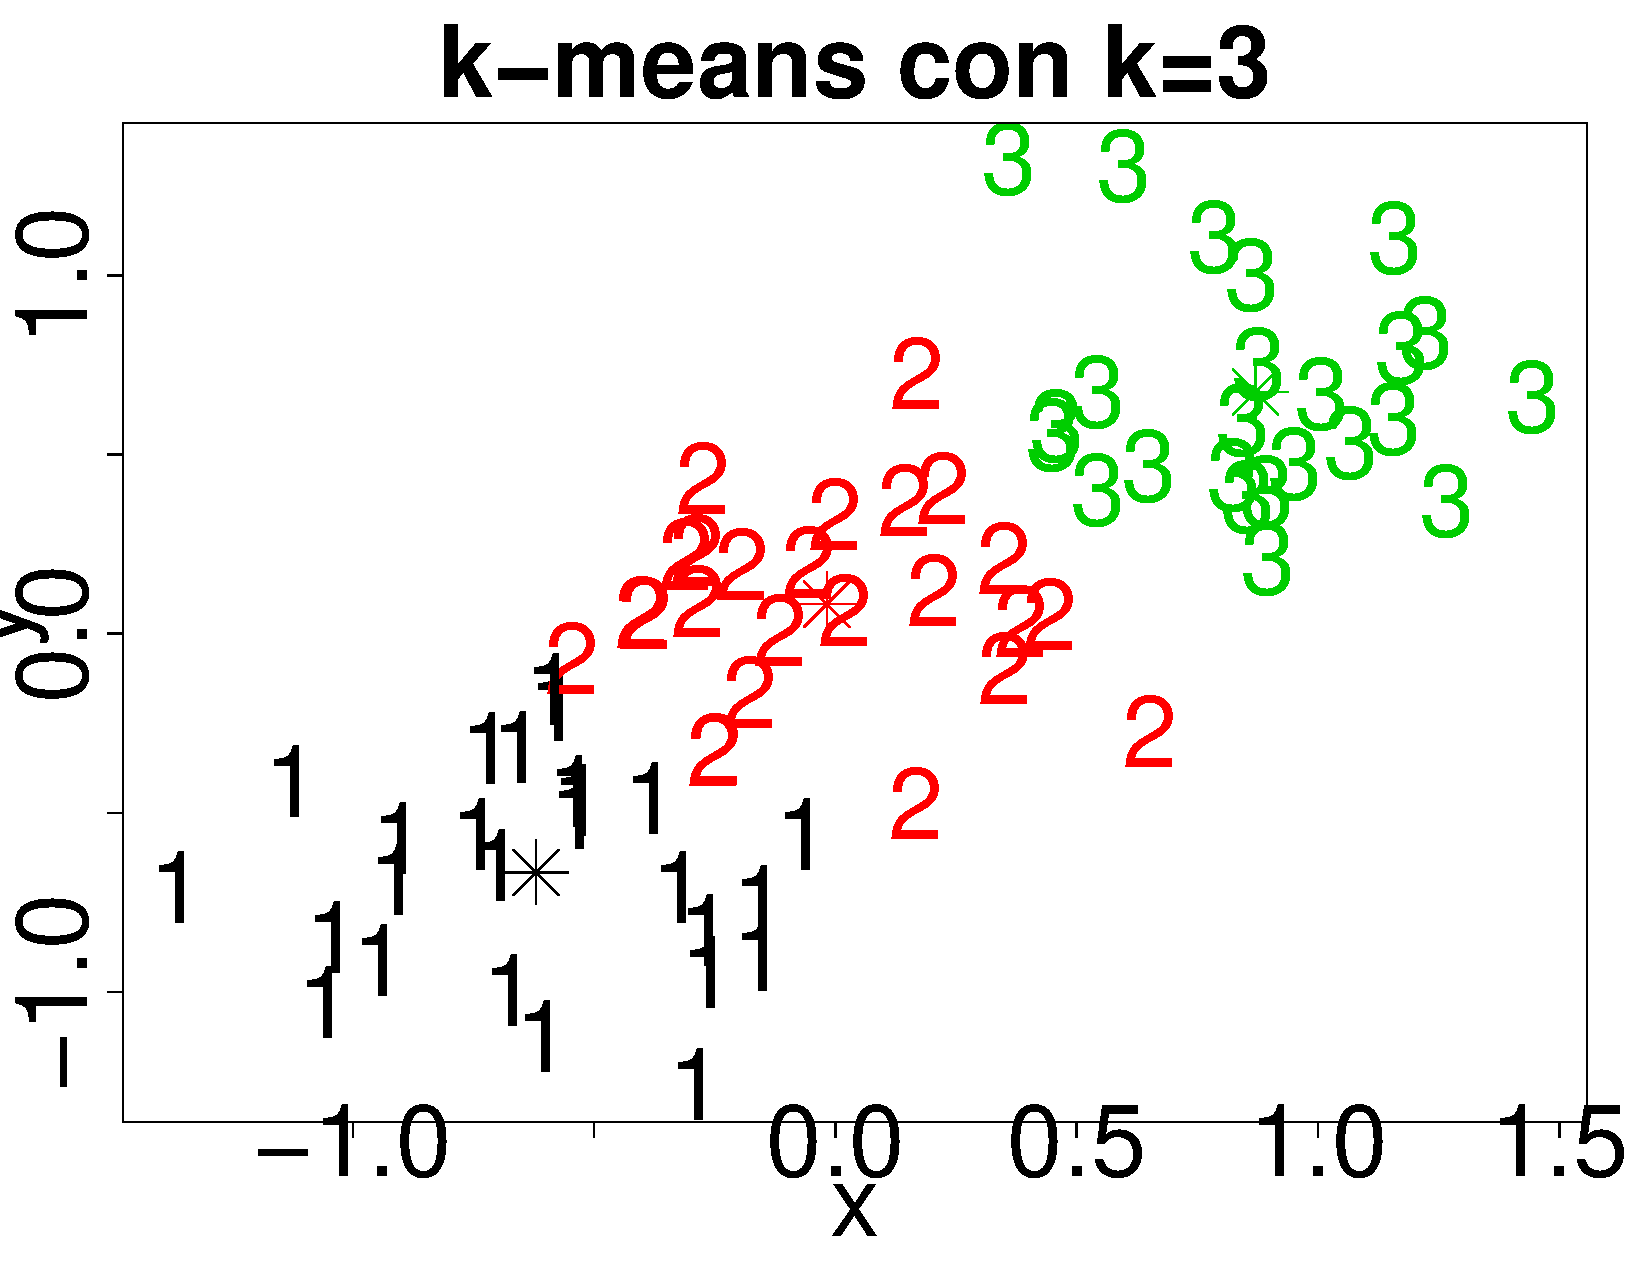
\includegraphics[width=0.8\textwidth]{ejemplo_kmeans_k3.pdf}
	
%	\centering	
%	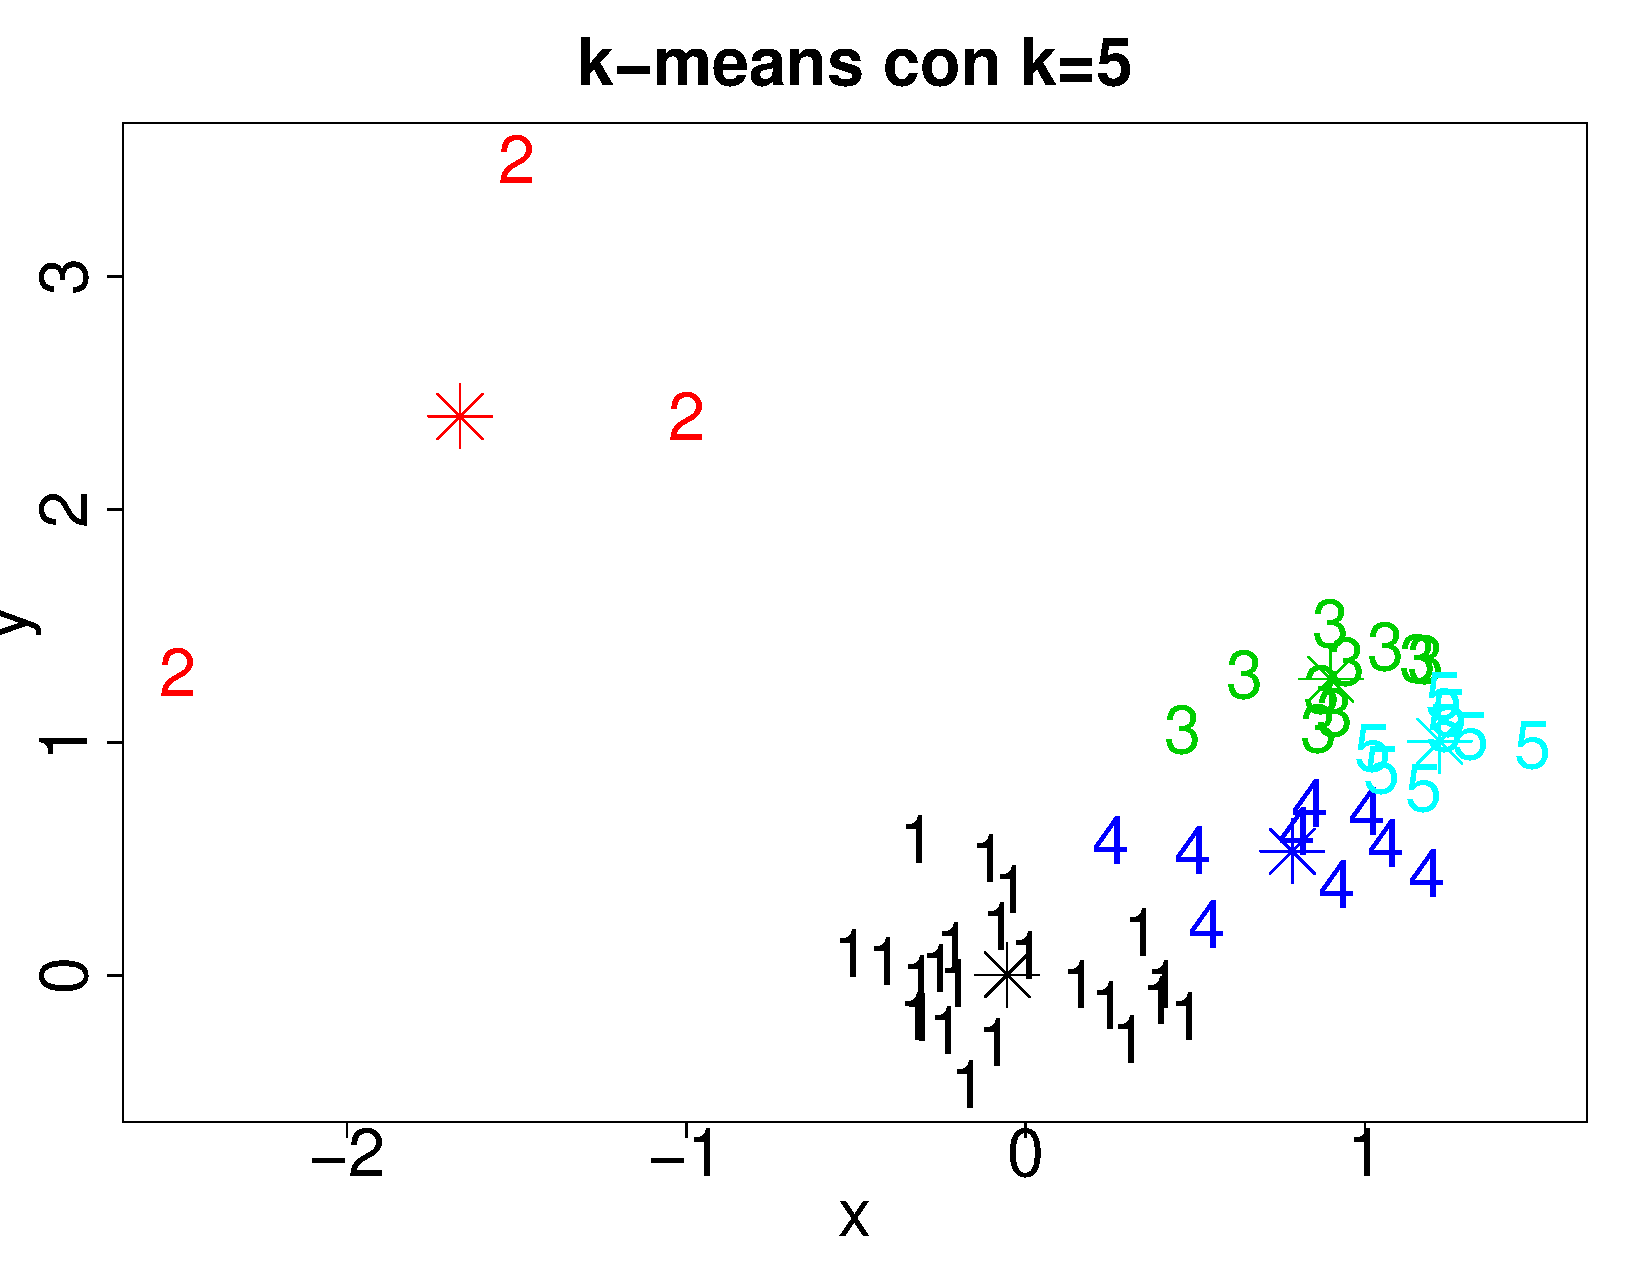
\includegraphics[width=0.8\textwidth]{ejemplo_kmeans_k5.pdf}	
%\end{columns}
%\end{frame}

%\begin{frame}\frametitle{Método de agrupamiento corte de árbol dinámico} 
%\centering
%\begin{itemize}
%\item Agrupamiento jerárquico.
%\item Utiliza la distancia de correlación.
%\item Se puede ``sintonizar'' la resolución del método. 
%\item DS1 particiones gruesas, con pocos grupos bien definidos.
%\item DS4 particiones finas, con muchos grupos más dispersos.
%\end{itemize}
%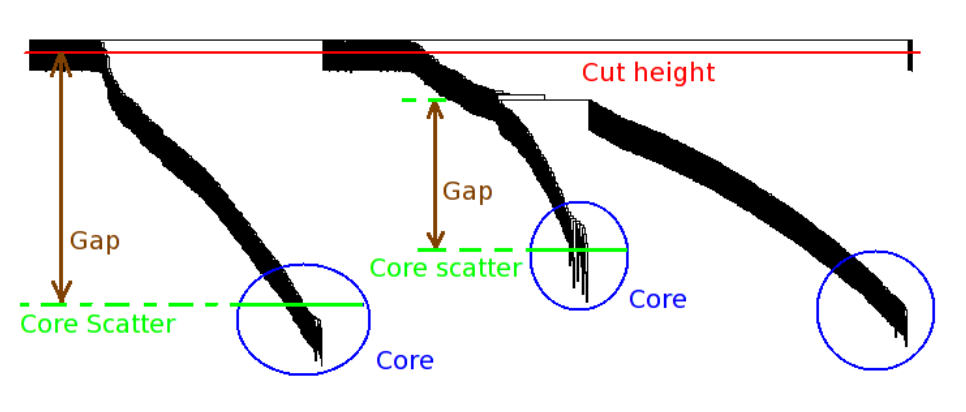
\includegraphics[height=0.55\textheight]{cut_tree_dynamic_ejemplo}	
%\end{frame}

\begin{frame}\frametitle{Métodos de agrupamiento} 

\begin{columns}[T]
\column{0.5\textwidth}
Método k-means
\begin{itemize}
	\item Busca estructuras compactas.
	\item La cantidad k de grupos debe ser fijada a priori.  
	\item Muy rápida ejecución. 	
\end{itemize}
\column{0.5\textwidth}
\end{columns}
\bigskip
\bigskip
\begin{columns}[T]
\column{0.5\textwidth}
Método corte de árbol dinámico
\begin{itemize}
	\item Agrupamiento jerárquico.
	\item El agrupamiento puede representarse mediante un dendrograma.
	\item Utiliza la distancia de correlación.
	\item La cantidad óptima de grupos k es decidida por el método.
\end{itemize}			
\column{0.5\textwidth}
    \centering
    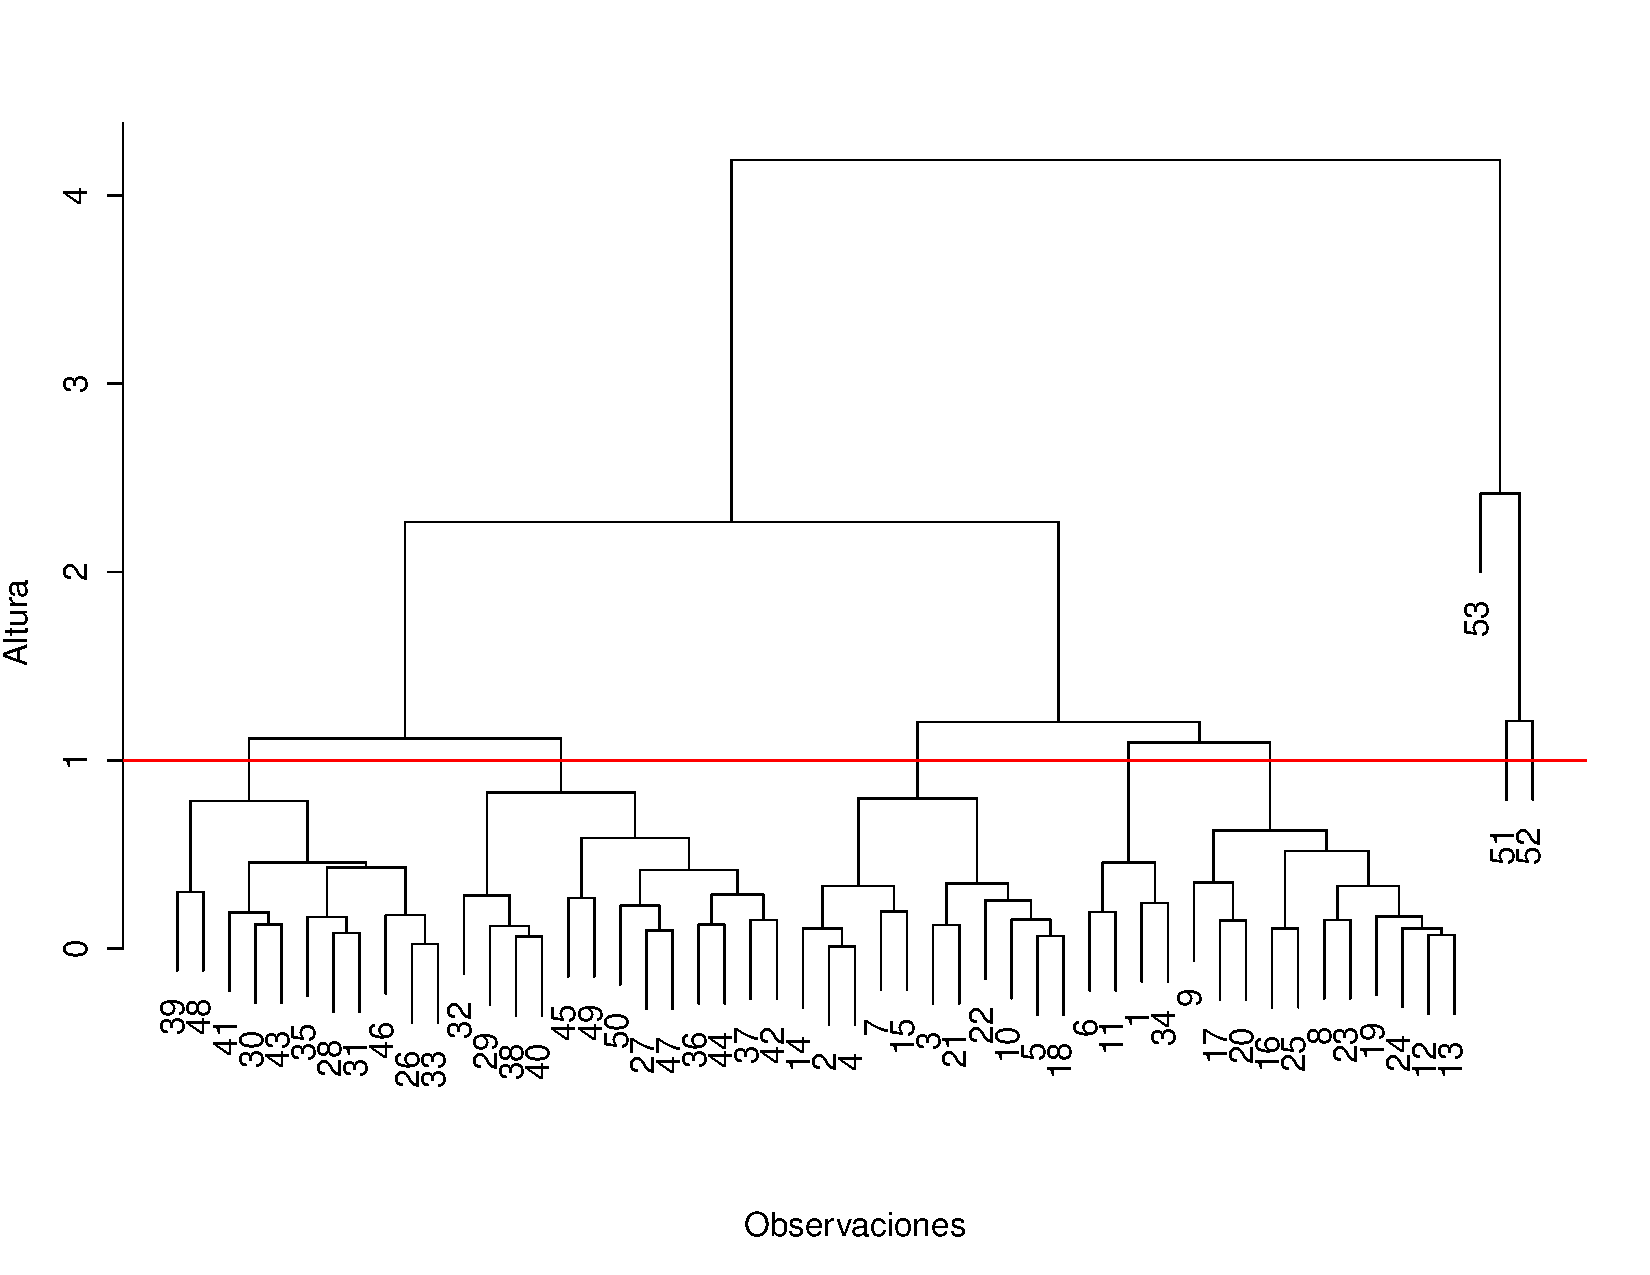
\includegraphics[width=1\textwidth]{dendrograma_muestra.pdf}
\end{columns}
\end{frame}

\begin{frame}\frametitle{Métodos de agrupamiento - ejemplos} 
\centering
\begin{columns}[T]
\column{0.5\textwidth}
    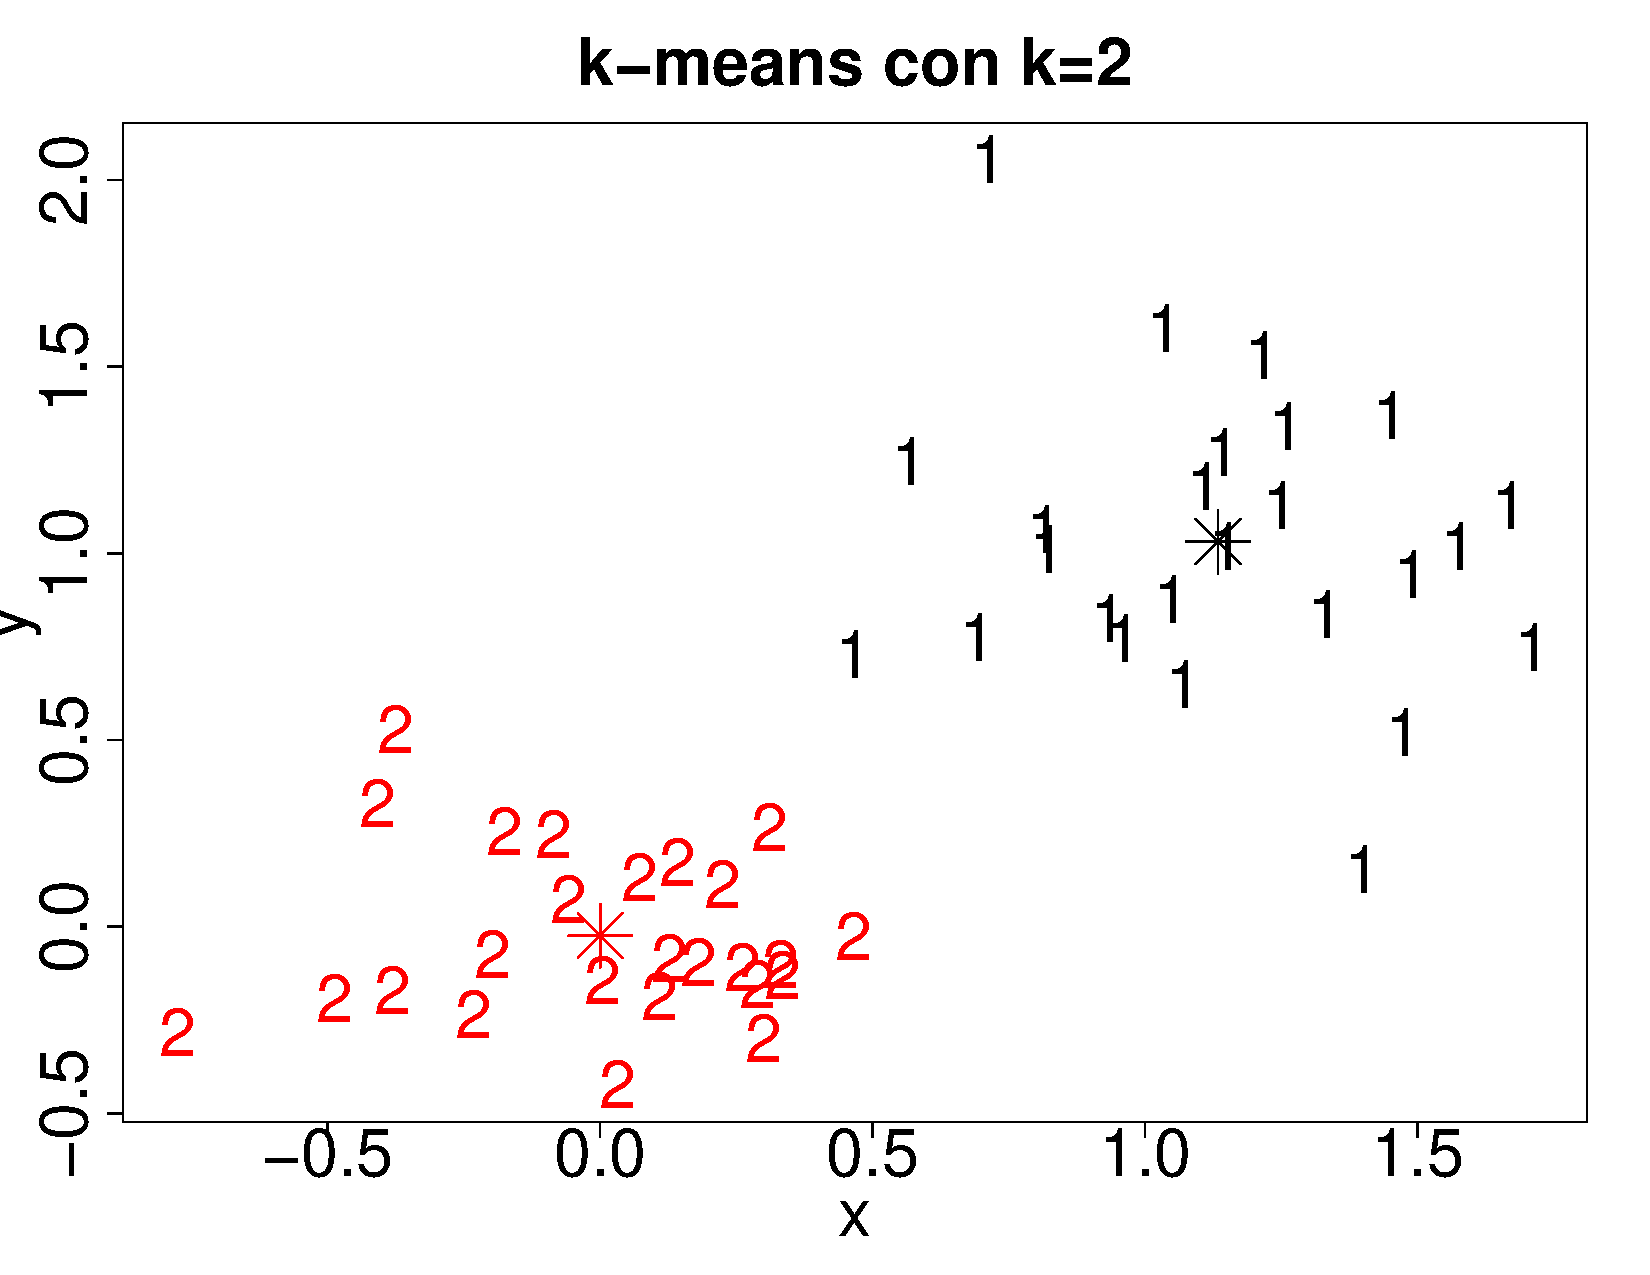
\includegraphics[width=0.8\textwidth]{ejemplo_kmeans_k2.pdf}
\column{0.5\textwidth}
    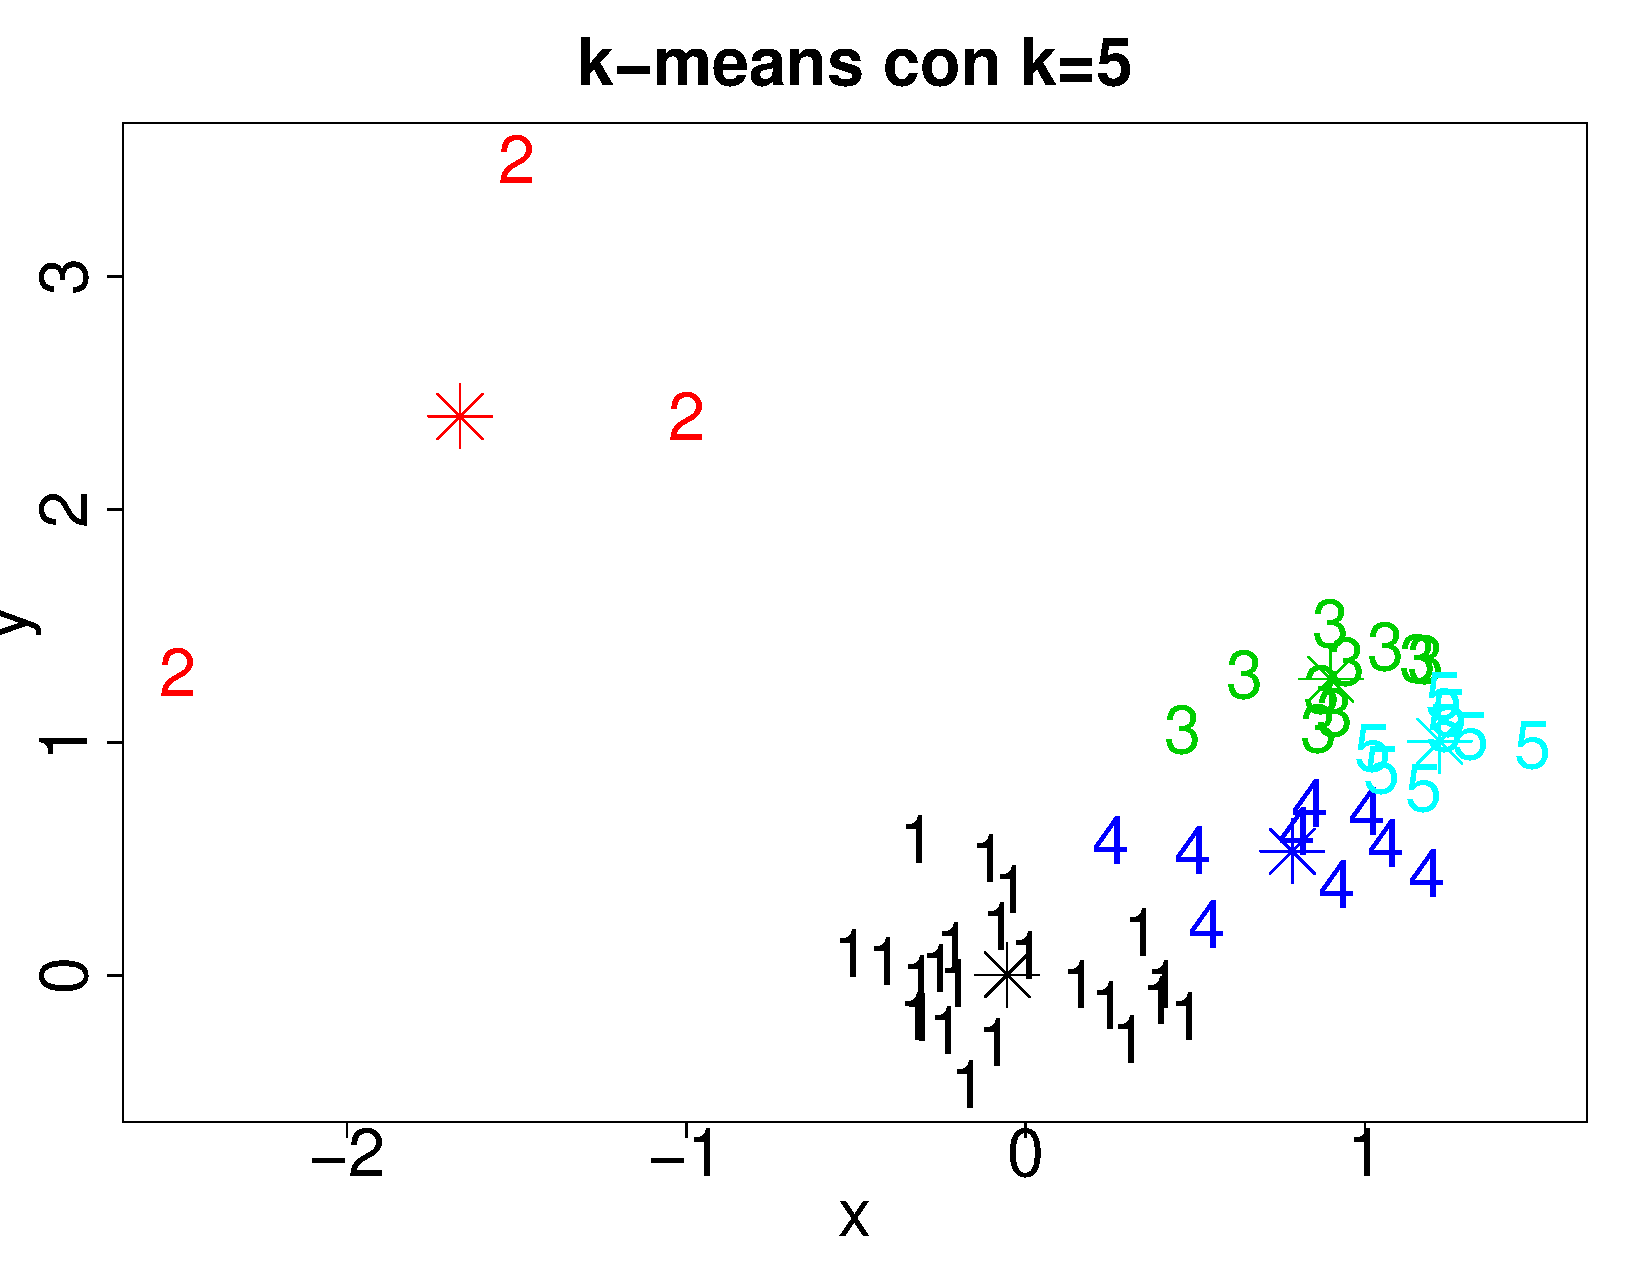
\includegraphics[width=0.8\textwidth]{ejemplo_kmeans_k5.pdf}
\end{columns}
\centering
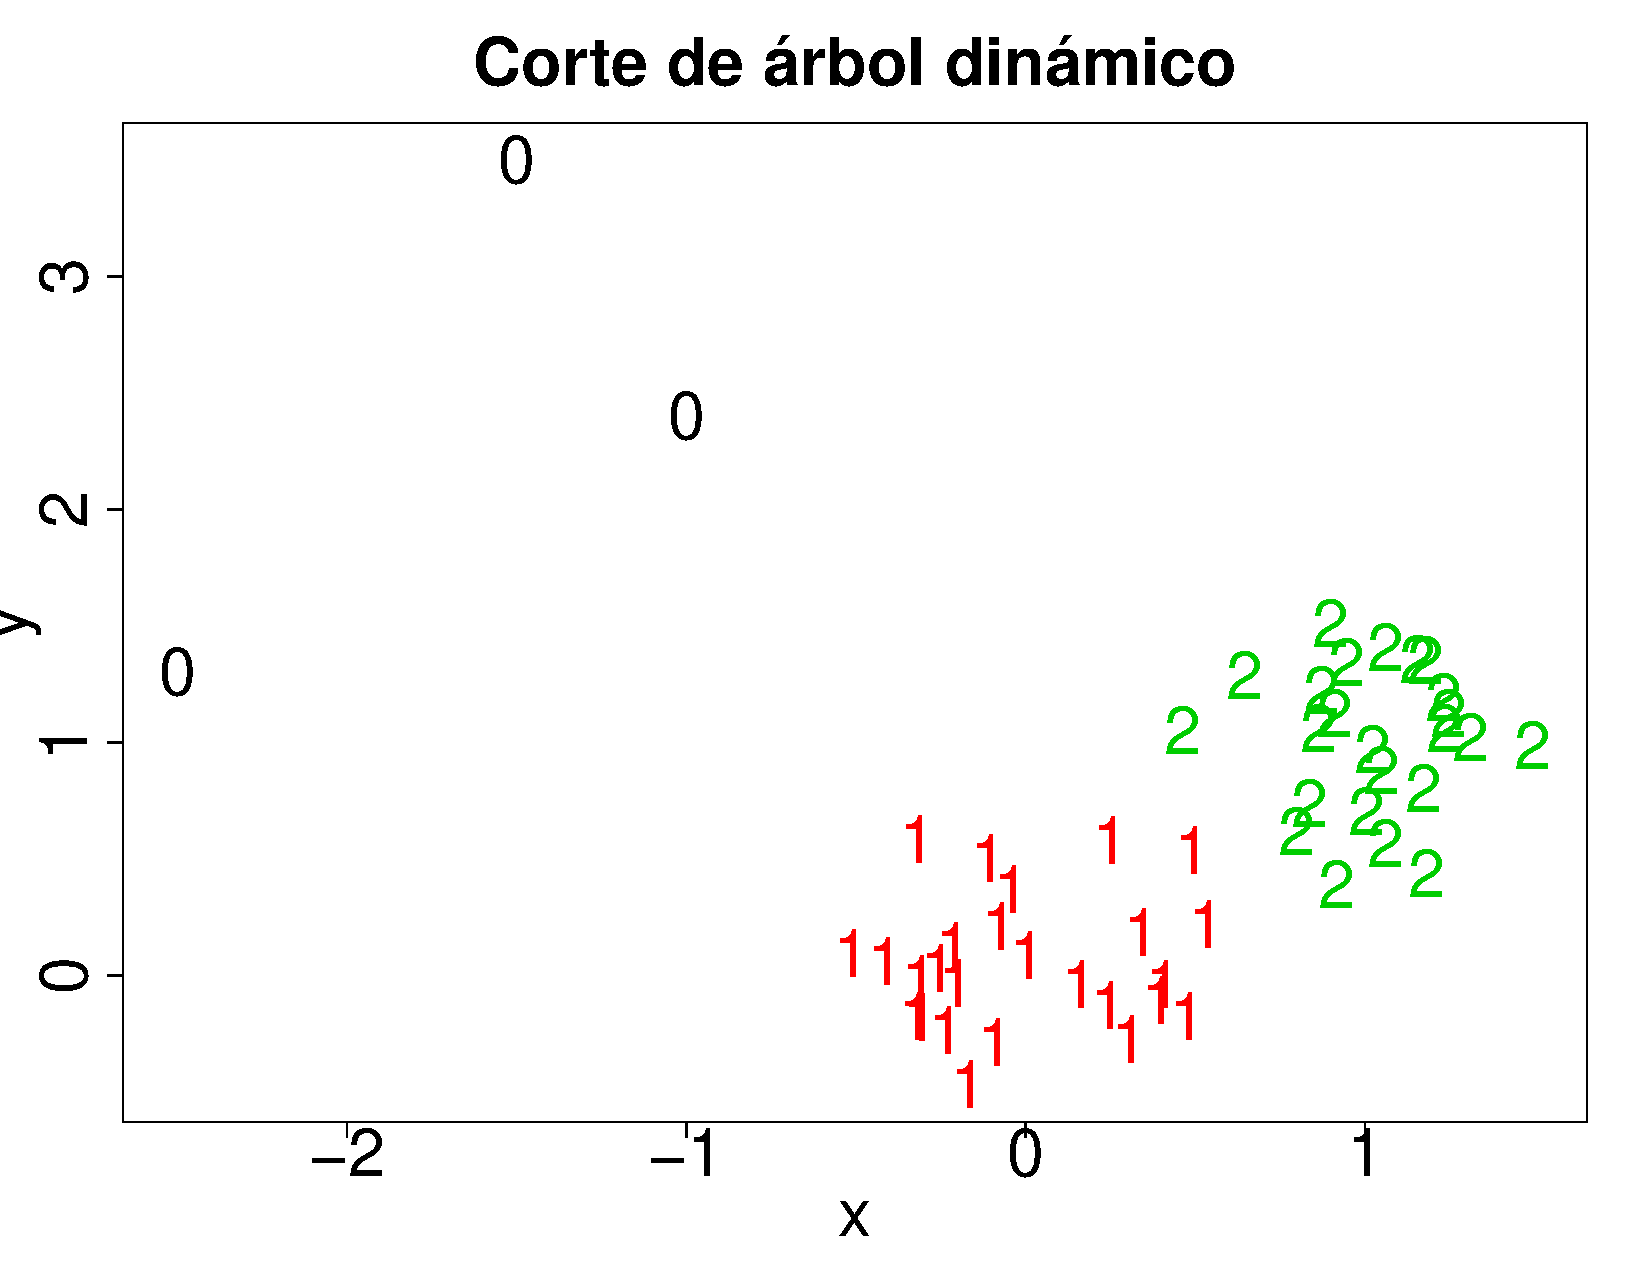
\includegraphics[width=0.4\textwidth]{ejemplo_dtc.pdf}    
\end{frame}

\subsection{Caracterización de particiones}
\begin{frame}\frametitle{Perfiles tratamiento ``Frío'' con k-means} 
\centering
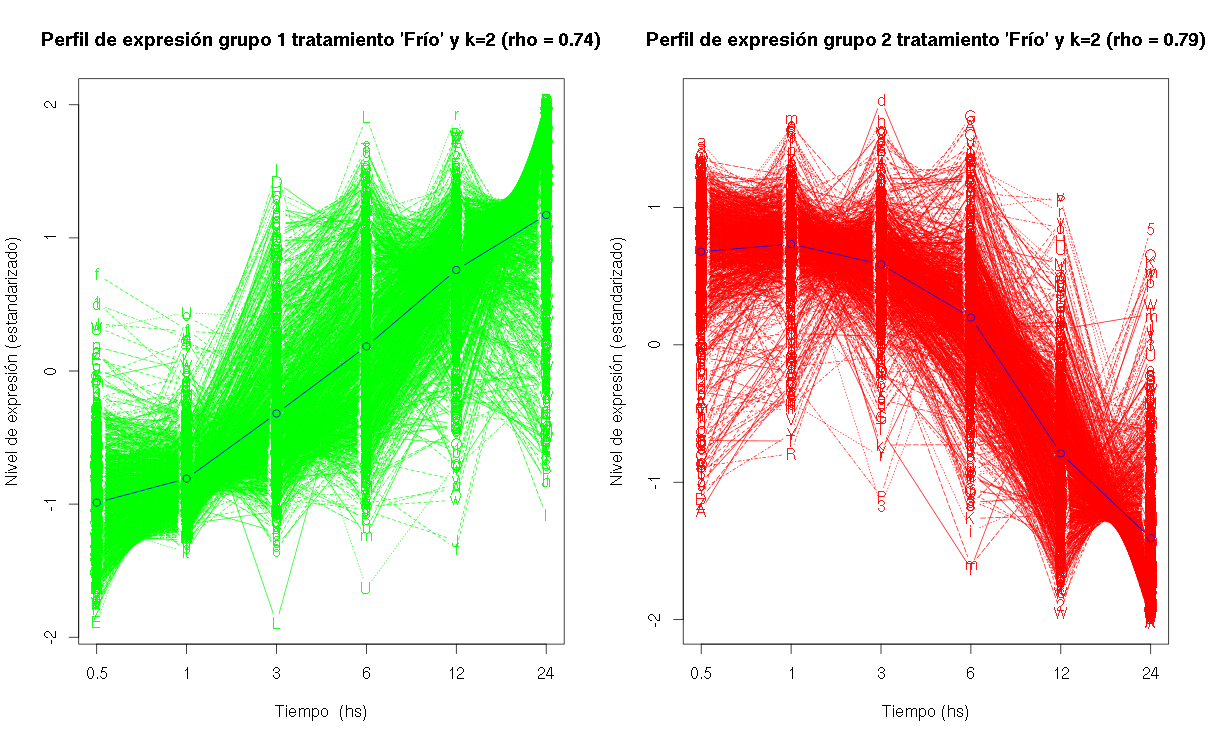
\includegraphics[width=1\textwidth]{perfiles_k_means}	
\end{frame}

\begin{frame}\frametitle{Perfiles tratamiento ``Frío'' con corte de árbol dinámico} 
\centering
A modo de ejemplo, los nueve perfiles más grandes de una partición de tratamiento ``Frío'' y DS1.\\
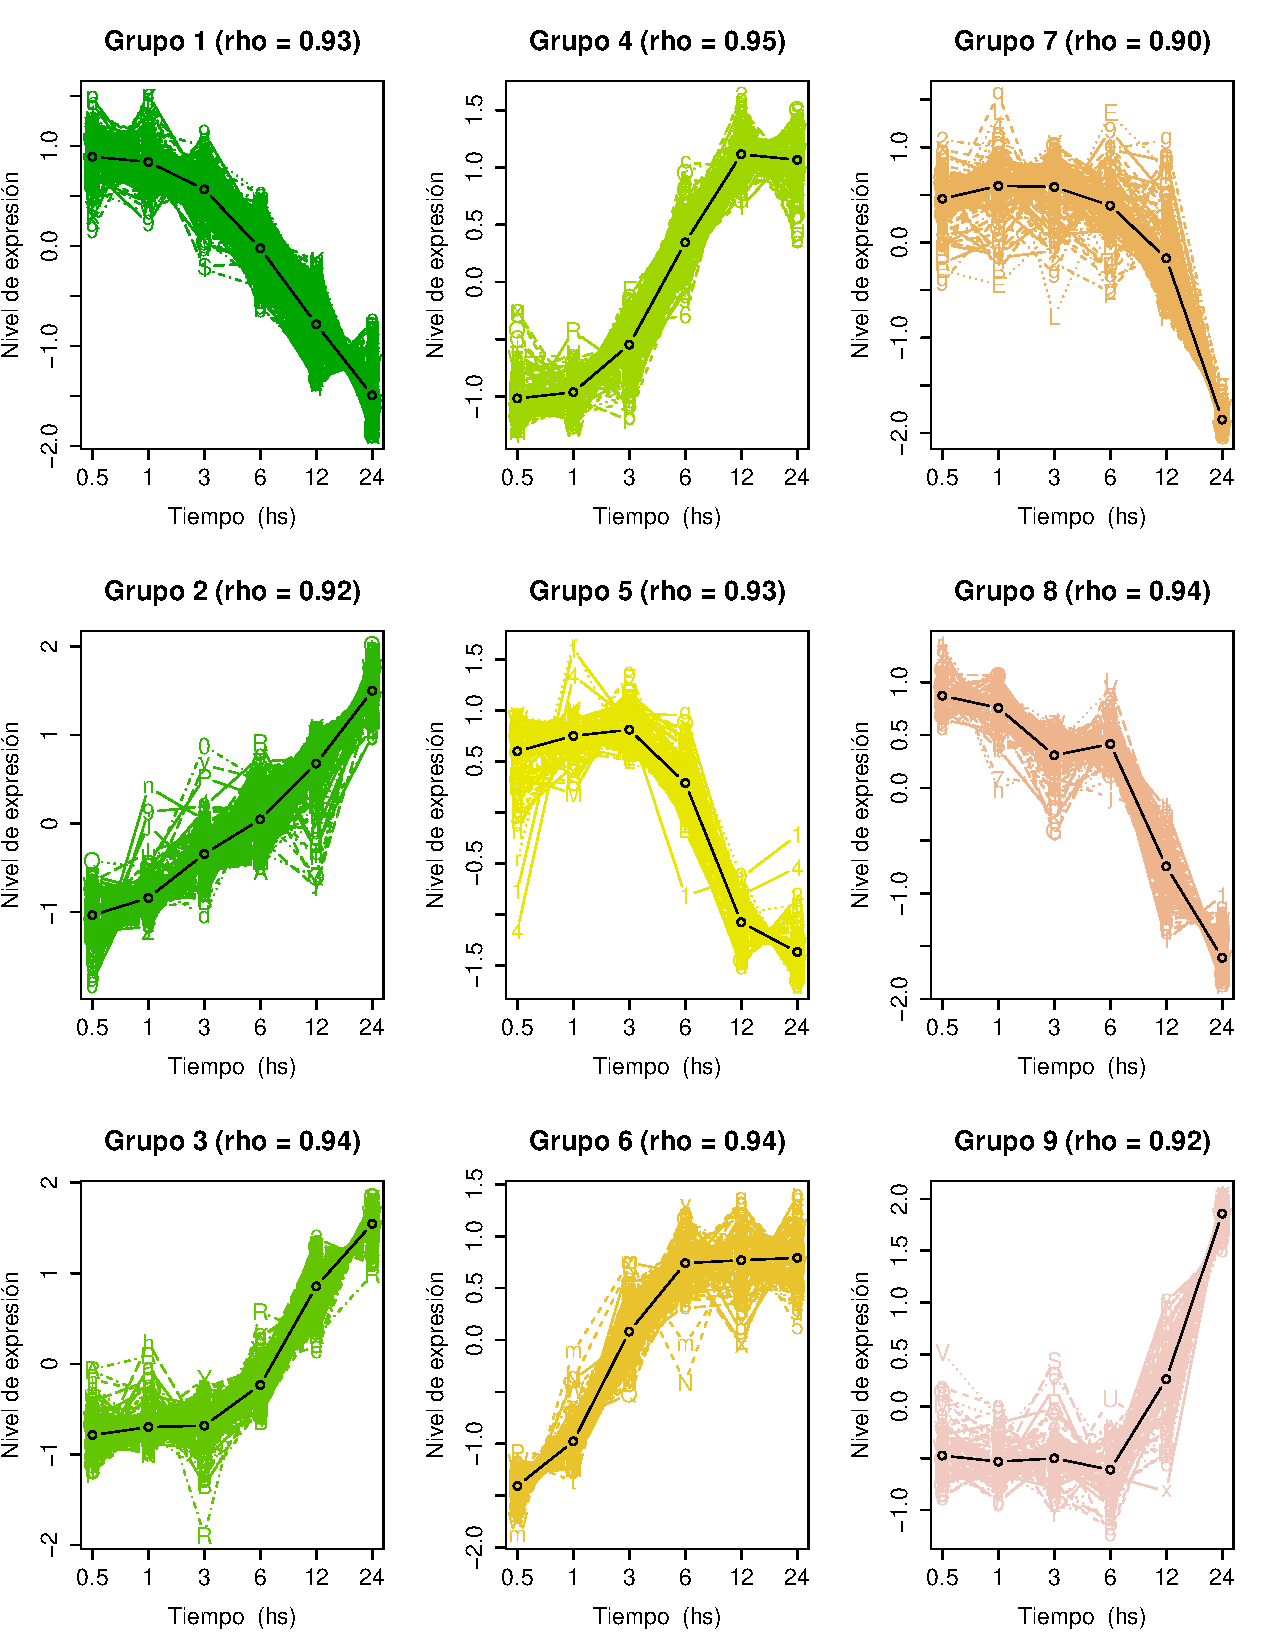
\includegraphics[width=0.8\textwidth, height=0.8\textheight]{perfiles_ds_1.pdf}	
\end{frame}

%\begin{frame}\frametitle{Caracterización de particiones corte de árbol dinámico} 
%\centering
%Correlación media por tamaño de grupo
%\begin{columns}[T]
%\column{0.5\textwidth}
%	\centering
%	DS1 (particiones más gruesas)
%	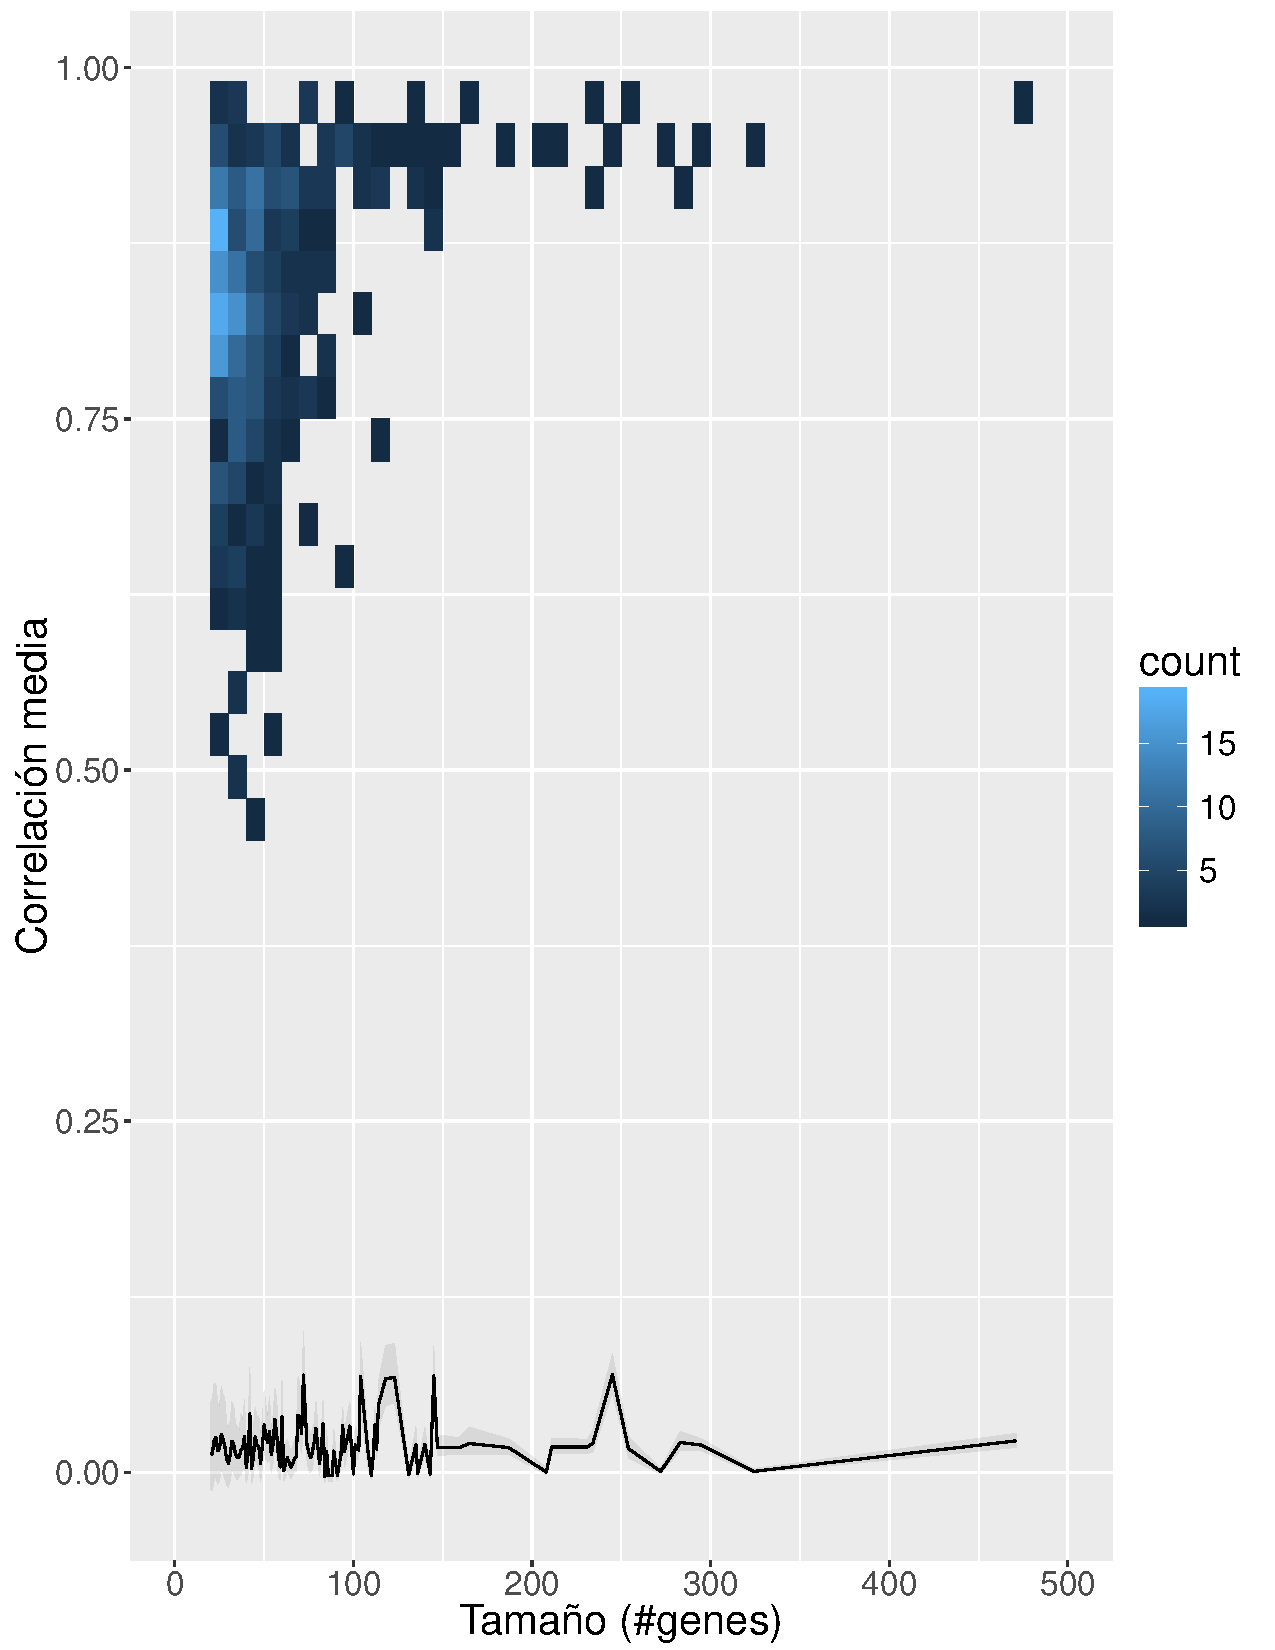
\includegraphics[width=0.9\textwidth]{correlacion_media_por_tamano_ds_1.pdf}	
%\column{0.5\textwidth}
%	\centering
%	DS4 (particiones más finas)
%	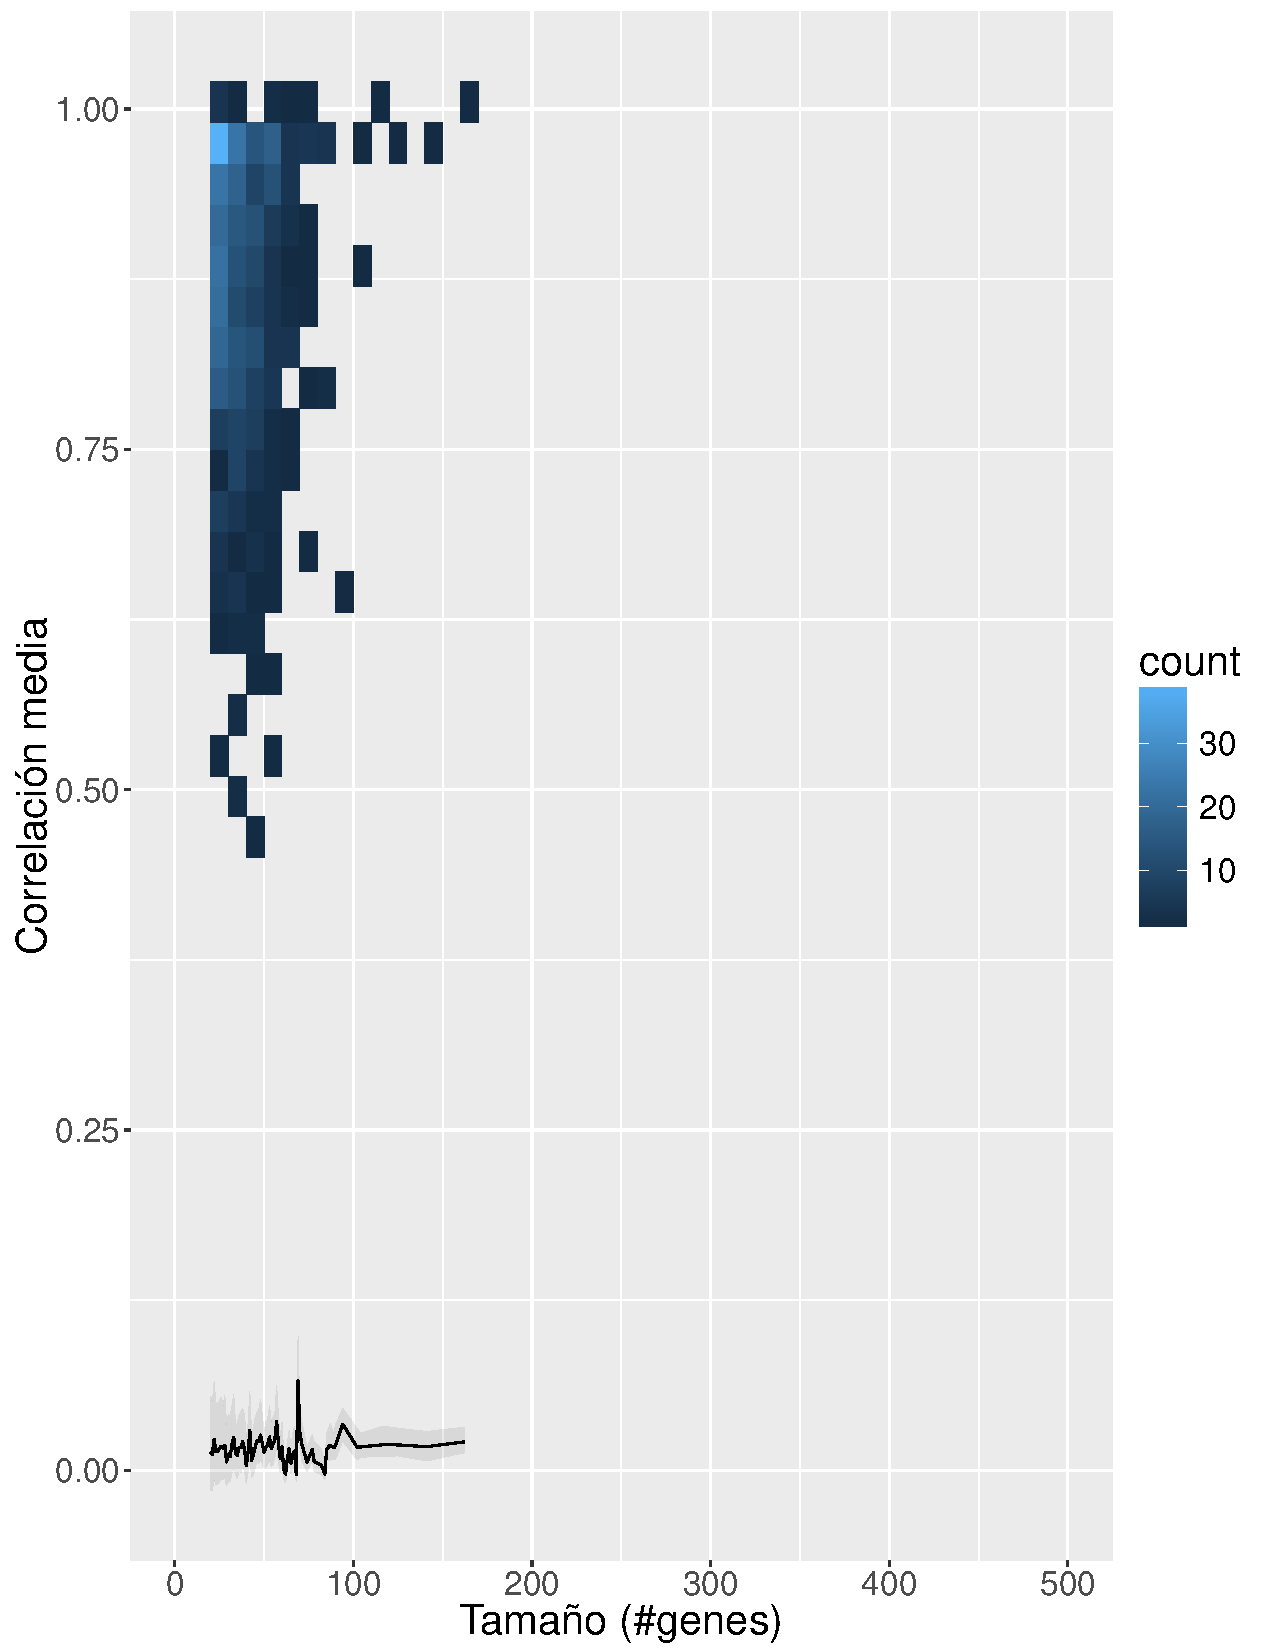
\includegraphics[width=0.9\textwidth]{correlacion_media_por_tamano_ds_4.pdf}	
%\end{columns}
%\end{frame}

%\begin{frame}\frametitle{Caracterización de granularidad de las particiones halladas} 
%\centering
%Fracción de grupos en una partición más fina dentro de grupos de una partición más gruesa (tratamiento ``Frío'')
%\begin{figure}
%    \centering
%	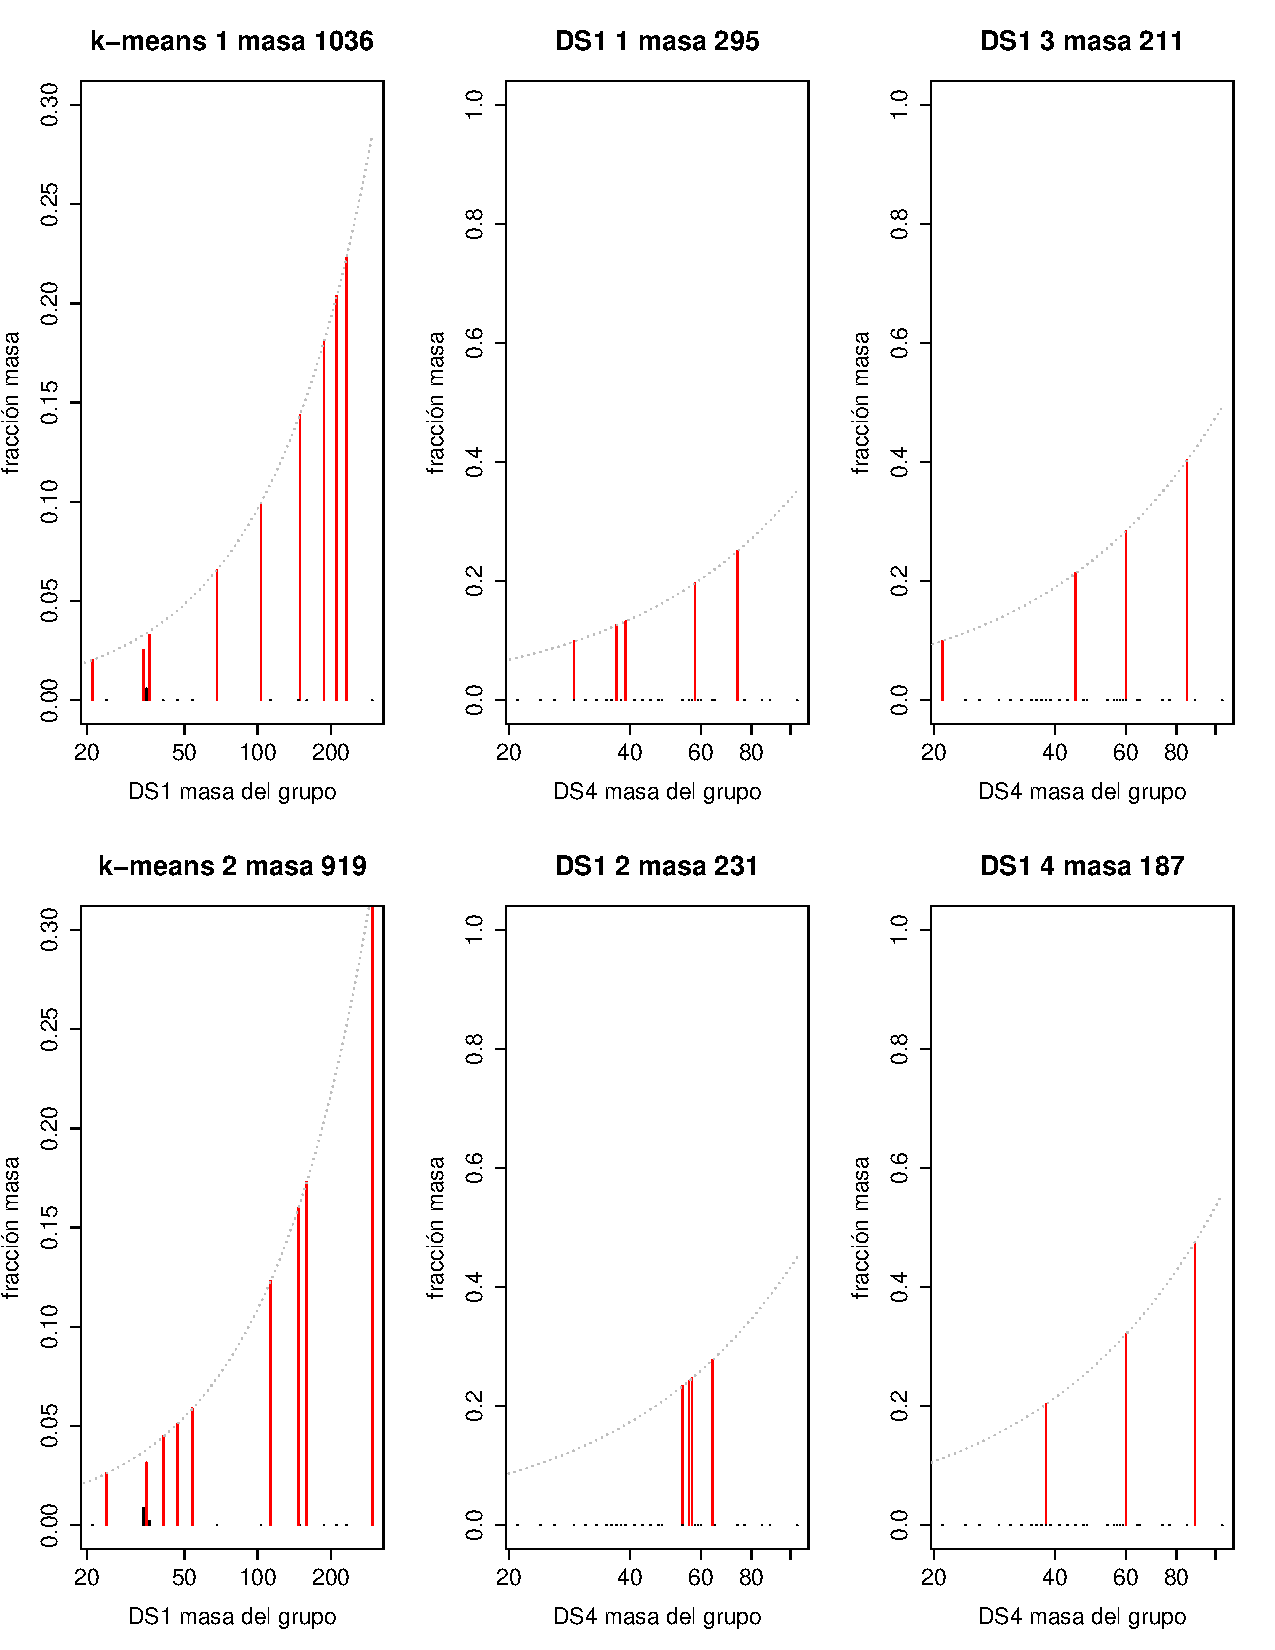
\includegraphics[height=1.6\textheight]{fraccion_de_km_en_ds1_en_ds4.pdf}	
%\end{figure}
%\end{frame}

\begin{frame}\frametitle{Granularidad de las particiones} 
Granularidad y resolución de los métodos
\bigskip
\begin{itemize}
\item Una partición $A$ es más fina que una partición $B$ si cada grupo de $A$ está contenido en un grupo de $B$.
\item Tenemos tres formas de realizar particiones de nuestros datos.
\item DS4 genera particiones más finas que DS1 y este a su vez que k-means.
\item Tenemos distintas maneras de encontrar estructura en nuestros datos y las distintas heterogeneidades aparecerán a distintas escalas.
\item Deberemos buscar la escala óptima a la que trabajar con este conjunto de datos y para eso vamos a pasar a un espacio de conocimiento biológico. 
\end{itemize}

\end{frame}

\section{Congruencia biológica}

\subsection{Ontología génica (GO)}
\begin{frame}\frametitle{Ontología génica (GO)}
\begin{columns}[T]
	\column{0.5\textwidth}
	\begin{itemize}
		\item Provee un vocabulario controlado de términos.
		\item Permite comparar y clasificar entidades biológicas.
		\item Tres ontologías: procesos biológicos (BP), componentes celulares (CC) y funciones moleculares (MF).
		\item Estructura de grafo acíclico dirigido (DAG).
		\item Cada nodo representa un témino que describe alguna función.
		\item Los nodos se unen entre si por medio de relaciones ``es un'' o ``es parte de''.
	\end{itemize}
	\column{0.5\textwidth}
	\centering
	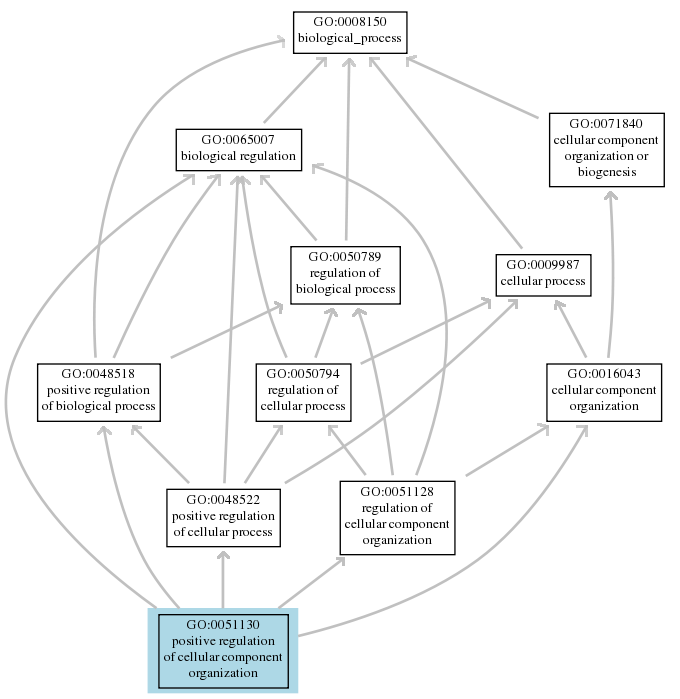
\includegraphics[width=1.1\textwidth]{ejemplo_de_go}	
	
	\medskip
	\Fontvi
	Un gen descrito por un término está ``anotado'' en ese término.	
\end{columns}
\end{frame}

\subsection{Cuantificando la congruencia biológica}
\begin{frame}\frametitle{Observables} 
\centering
Buscamos cuantificar la congruencia biológica de las particiones halladas
\bigskip
\begin{columns}[T]
	\column{0.5\textwidth}
	Densidad de interacción:\\
	\bigskip
	\begin{equation}
		ID(GO_j) = \frac{NE(GO_j)}{N(GO_j)}
	\end{equation}
	\bigskip
	Con $NE(GO_j)$ la cantidad de pares de genes anotados en $GO_j$ que se encuentran juntos en un mismo grupo 	transcripcional $C_x$ y $N(GO_j)$ la cantidad de pares de genes anotados en $GO_j$.
	\column{0.5\textwidth}
	Indice de homogeneidad biológica:\\
	\bigskip
	\begin{equation}
		BHI_j = \frac{1}{n_j(n_j-1)}\sum\limits_{x\neq y\in D_j}I(C(x)=C(y))
	\end{equation}
	\bigskip	
	Con $n_j$ la cantidad de genes anotados en el grupo $D_j$.\\
	La función indicadora $I(C(x)=C(y))$ que toma el valor $1$ si hay al menos una clase en donde ambos genes estén anotados, y $0$ en caso contrario.
\end{columns}
\end{frame}

\begin{frame}\frametitle{Densidad de interacción} 
\begin{columns}[T]
	\column{0.3\textwidth}
	\Fontvi
	\begin{enumerate}
	\item Términos mas específicos presentan mayor ID en una relación decreciente.
	\item DS1 presenta mayor congruencia biológica que DS4. Indicio acerca de la escala apropiada.
	\item Ambos presentan mayor congruencia biológica que control nulo.
	\item Los agrupamientos inducidos por otra información presentan mayor congruencia que los inducidos por expresión.
	\end{enumerate}
	\column{0.7\textwidth}
	\begin{figure}
	    	\centering
		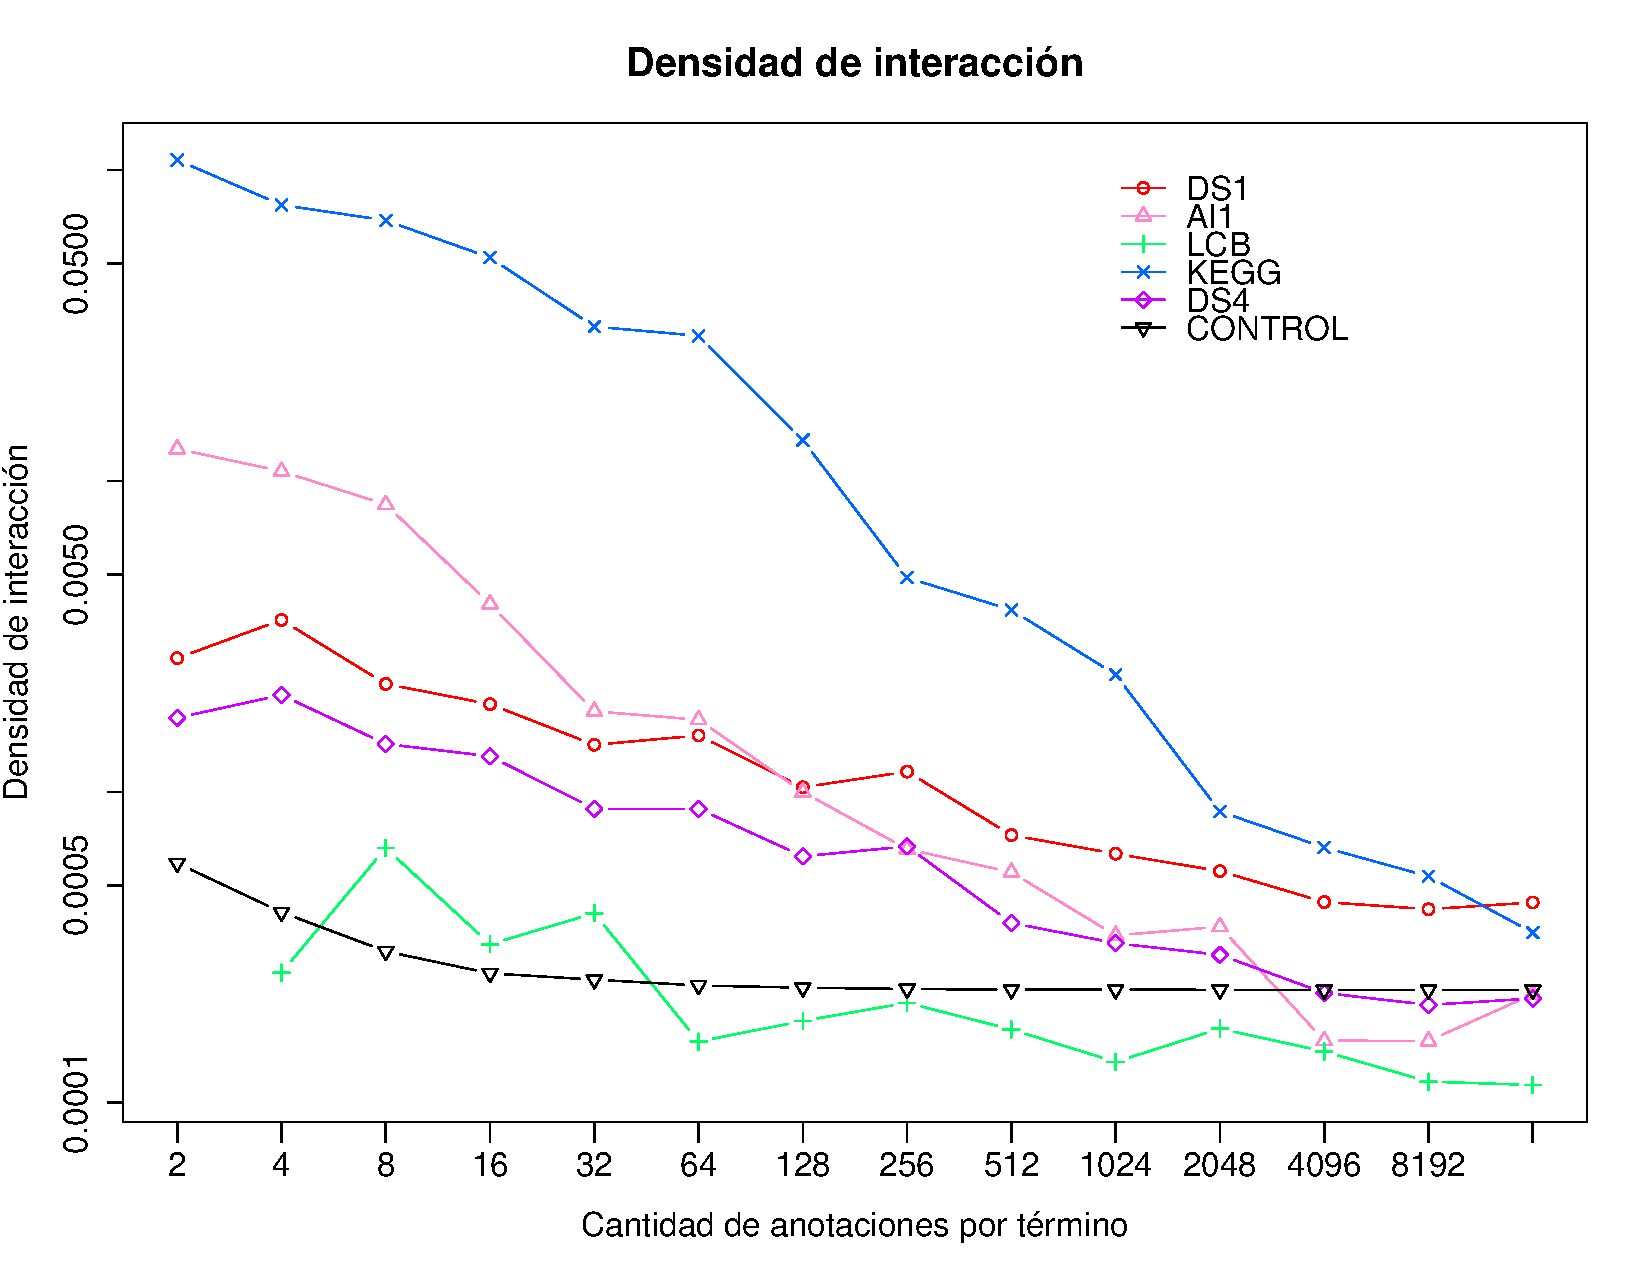
\includegraphics[width=1\textwidth]{interacting_densities_bpb.pdf}
	\end{figure}
\end{columns}
\end{frame}

\begin{frame}\frametitle{Indice de homogeneidad biológica} 
\begin{figure}
    	\centering
	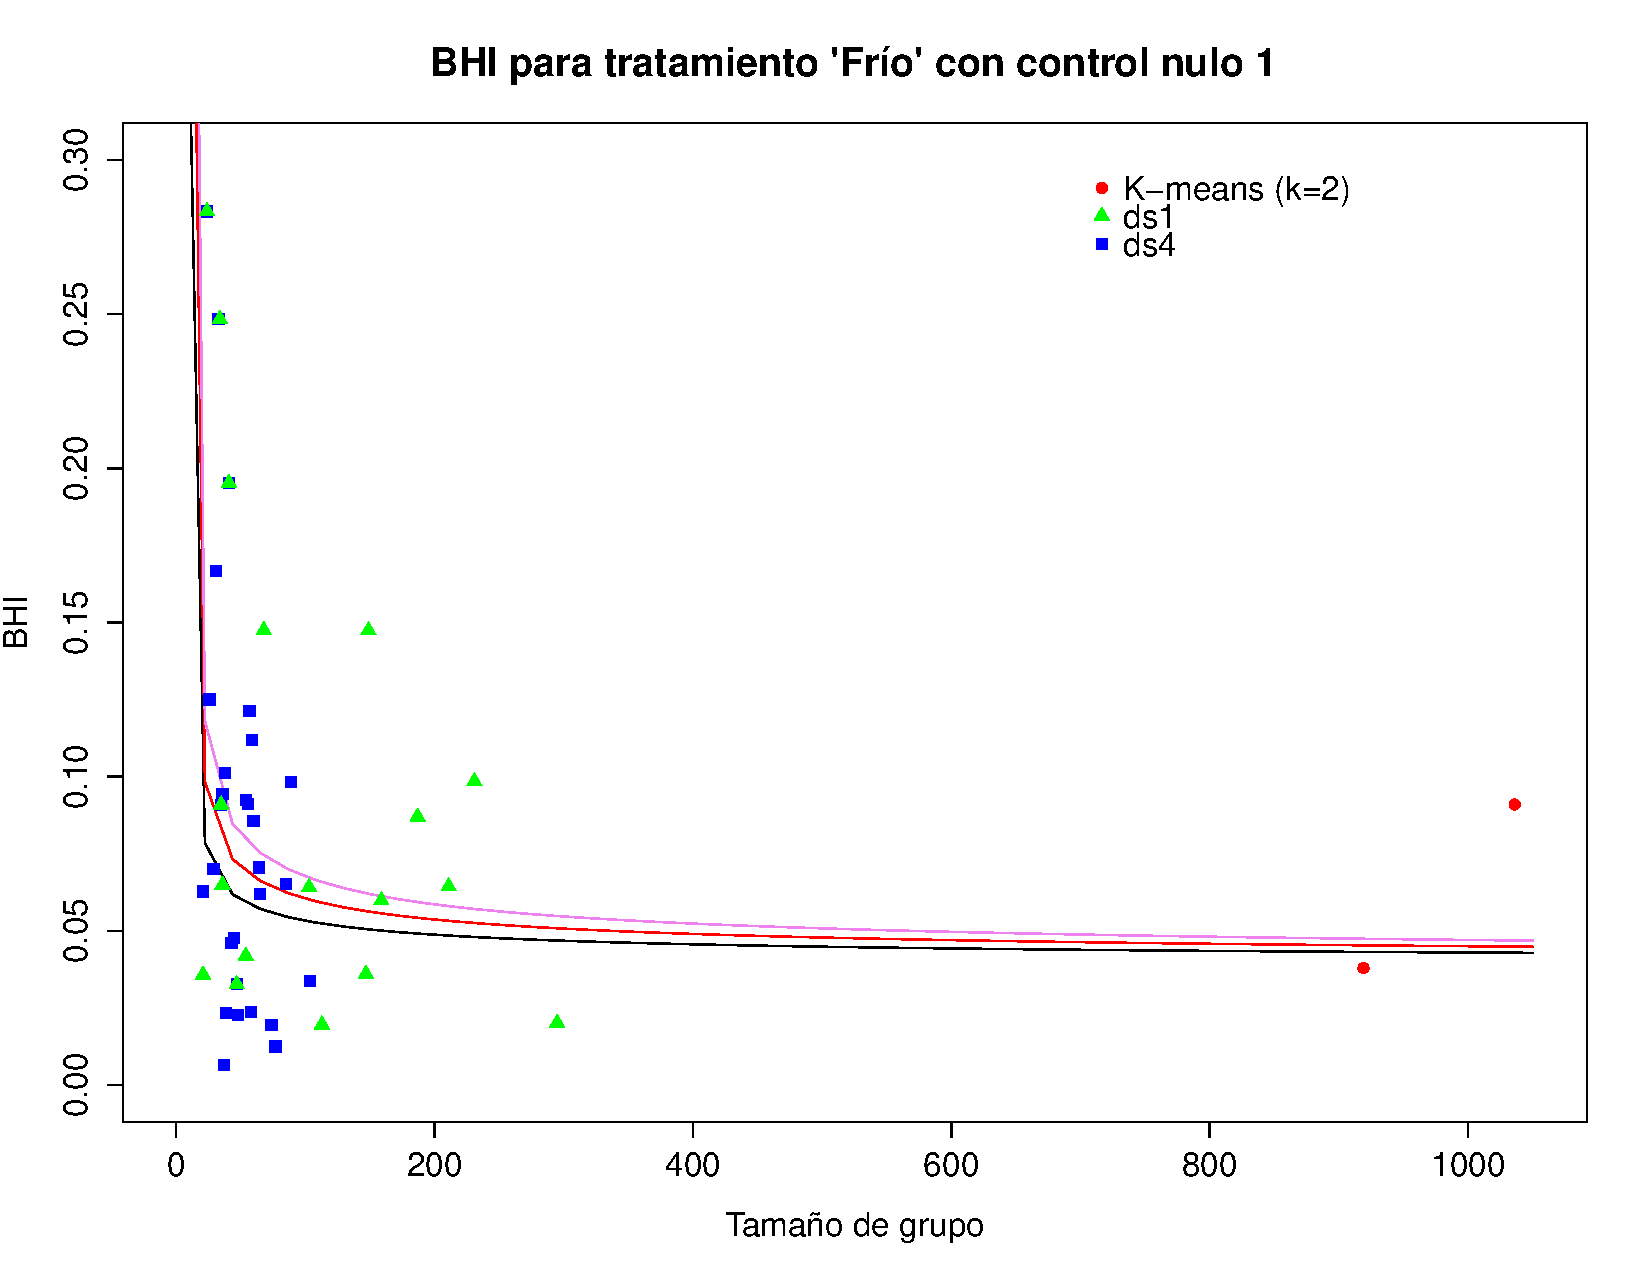
\includegraphics[width=0.78\textwidth]{bhi_km_ds1_ds4_control1.pdf}
\end{figure}
\Fontvi
\centering
Grupos altamente coherentes pero de baja calidad de BHI. No tienen soporte biológico.
\end{frame}

\section{Coherencia entre métricas}

\subsection{Métrica en GO}
\begin{frame}\frametitle{Similaridad entre genes en GO}
\centering
Podemos definir similaridades entre genes en el espacio GO\\
\bigskip
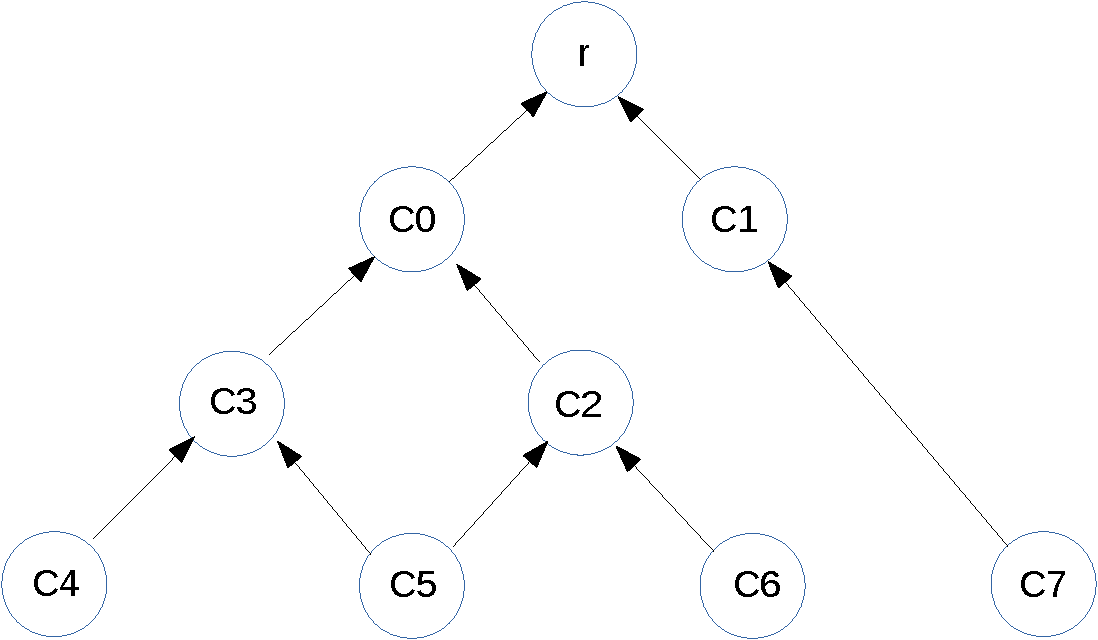
\includegraphics[width=0.5\textwidth]{dag.pdf}
\\\bigskip
Utilizando la similaridad entre términos:
\begin{equation}
	Sim_{res}(c_i, c_j) = \max\limits_{c \in S(c_i, c_j)}(-log_2[P(c)]) = IC(MICA[c_i, c_j])
\end{equation}
\end{frame}

\subsection{KTA global}
\begin{frame}\frametitle{KTA global} 
La noción de similaridad de a pares en cada espacio esta dada en términos de una función $k$ llamada kernel tal que
\begin{equation}
	K = K_{ij} = k(x_i, x_j)
\end{equation}
\bigskip
El KTA de un kernel $k_1$ con respecto a un kernel $k_2$ del conjunto $C$ cuantifica la similaridad entre dos espacios y se define como:
\begin{equation}
	\hat{A}(C, k_1, k_2) = \frac{\langle K_1, K_2 \rangle _F}{\sqrt{\langle K_1, K_1 \rangle _F \langle K_2, K_2 \rangle _F}}
\end{equation}
con $\langle K_1, K_1 \rangle _F = \sum_{i,j=1}^m K_1(x_i, x_j)K_2(x_i, x_j)$ es el producto interno de Frobenius.\\
Intiutivamente, si $\langle K_1, K_1 \rangle$ es grande, ambos kernels son coherentes.
\end{frame}

\begin{frame}\frametitle{KTA global} 
\centering
KTA global entre expresión y ontología BPB con control nulo
\begin{figure}
    	\centering
	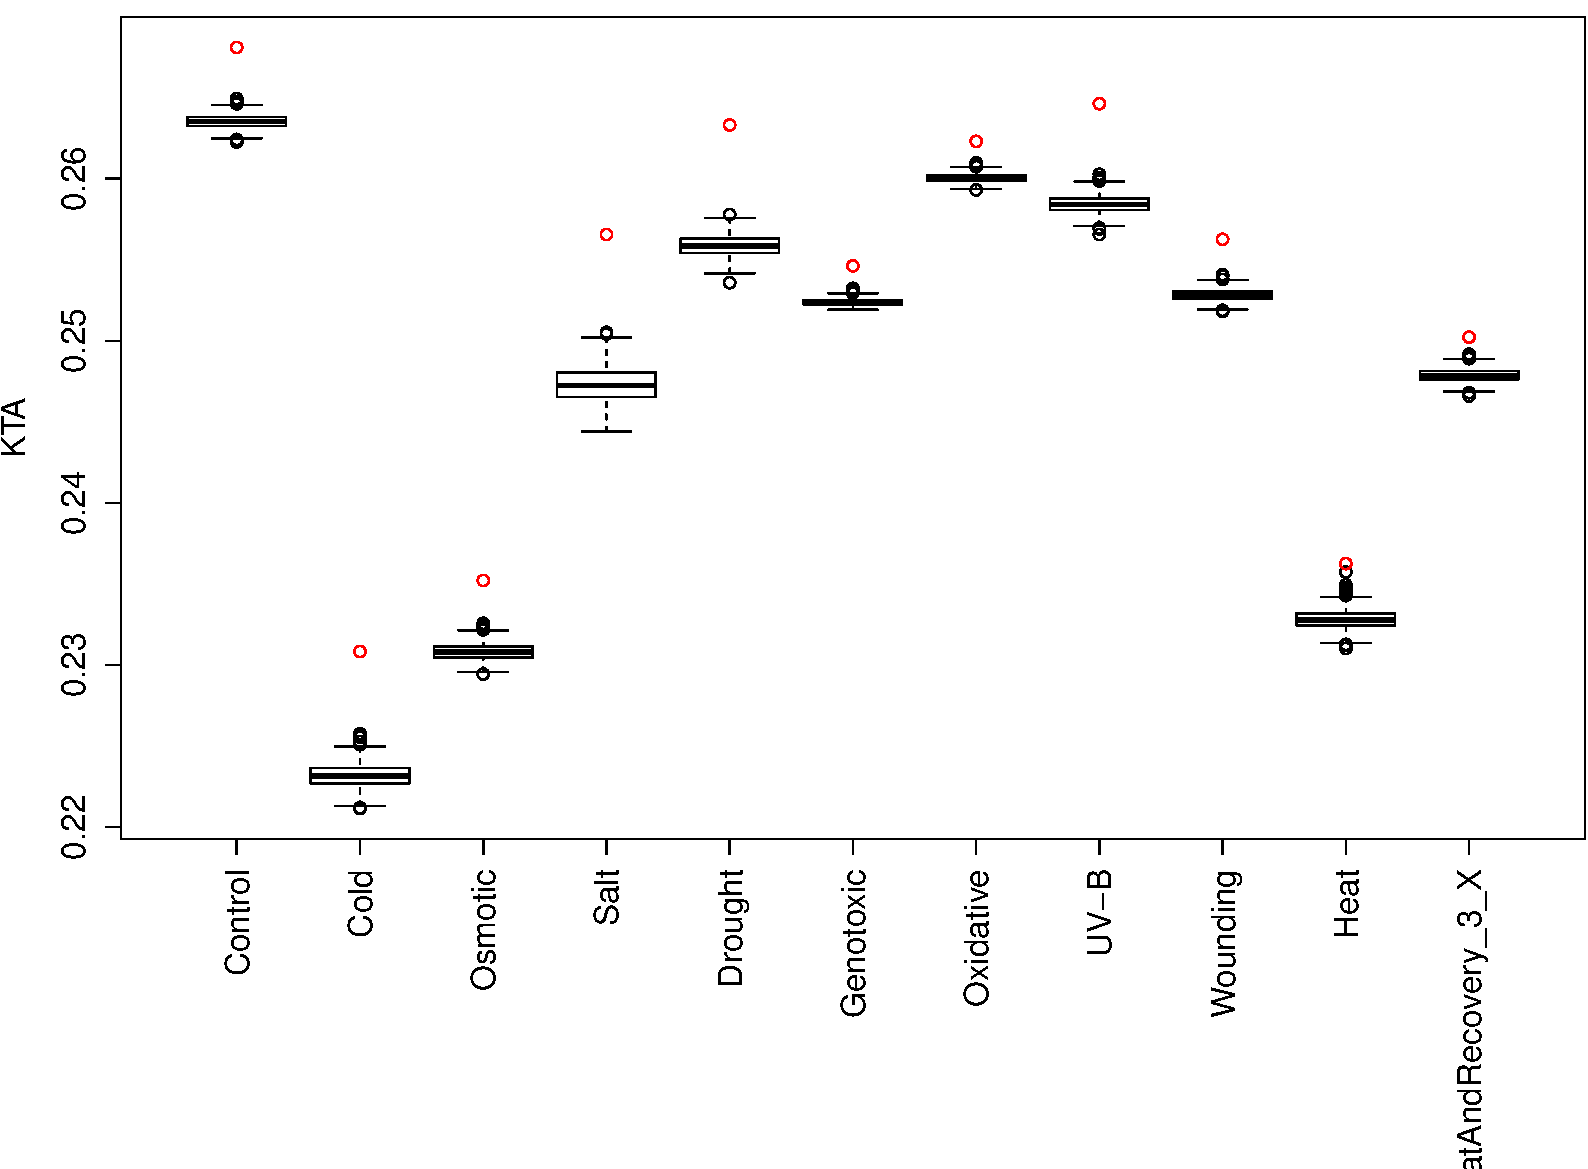
\includegraphics[width=0.8\textwidth]{kta_global_bpb.pdf}
\end{figure}
\centering
\end{frame}

\subsection{Modulación de heterogeneidades
transcripcionales con GO}
%\begin{frame}\frametitle{Red 30 primeros vecinos mutuos} 
%\bigskip
%\begin{columns}[T]
%	\column{0.5\textwidth}
%	\centering
%   Distribución de grado\\	
%  \bigskip
%    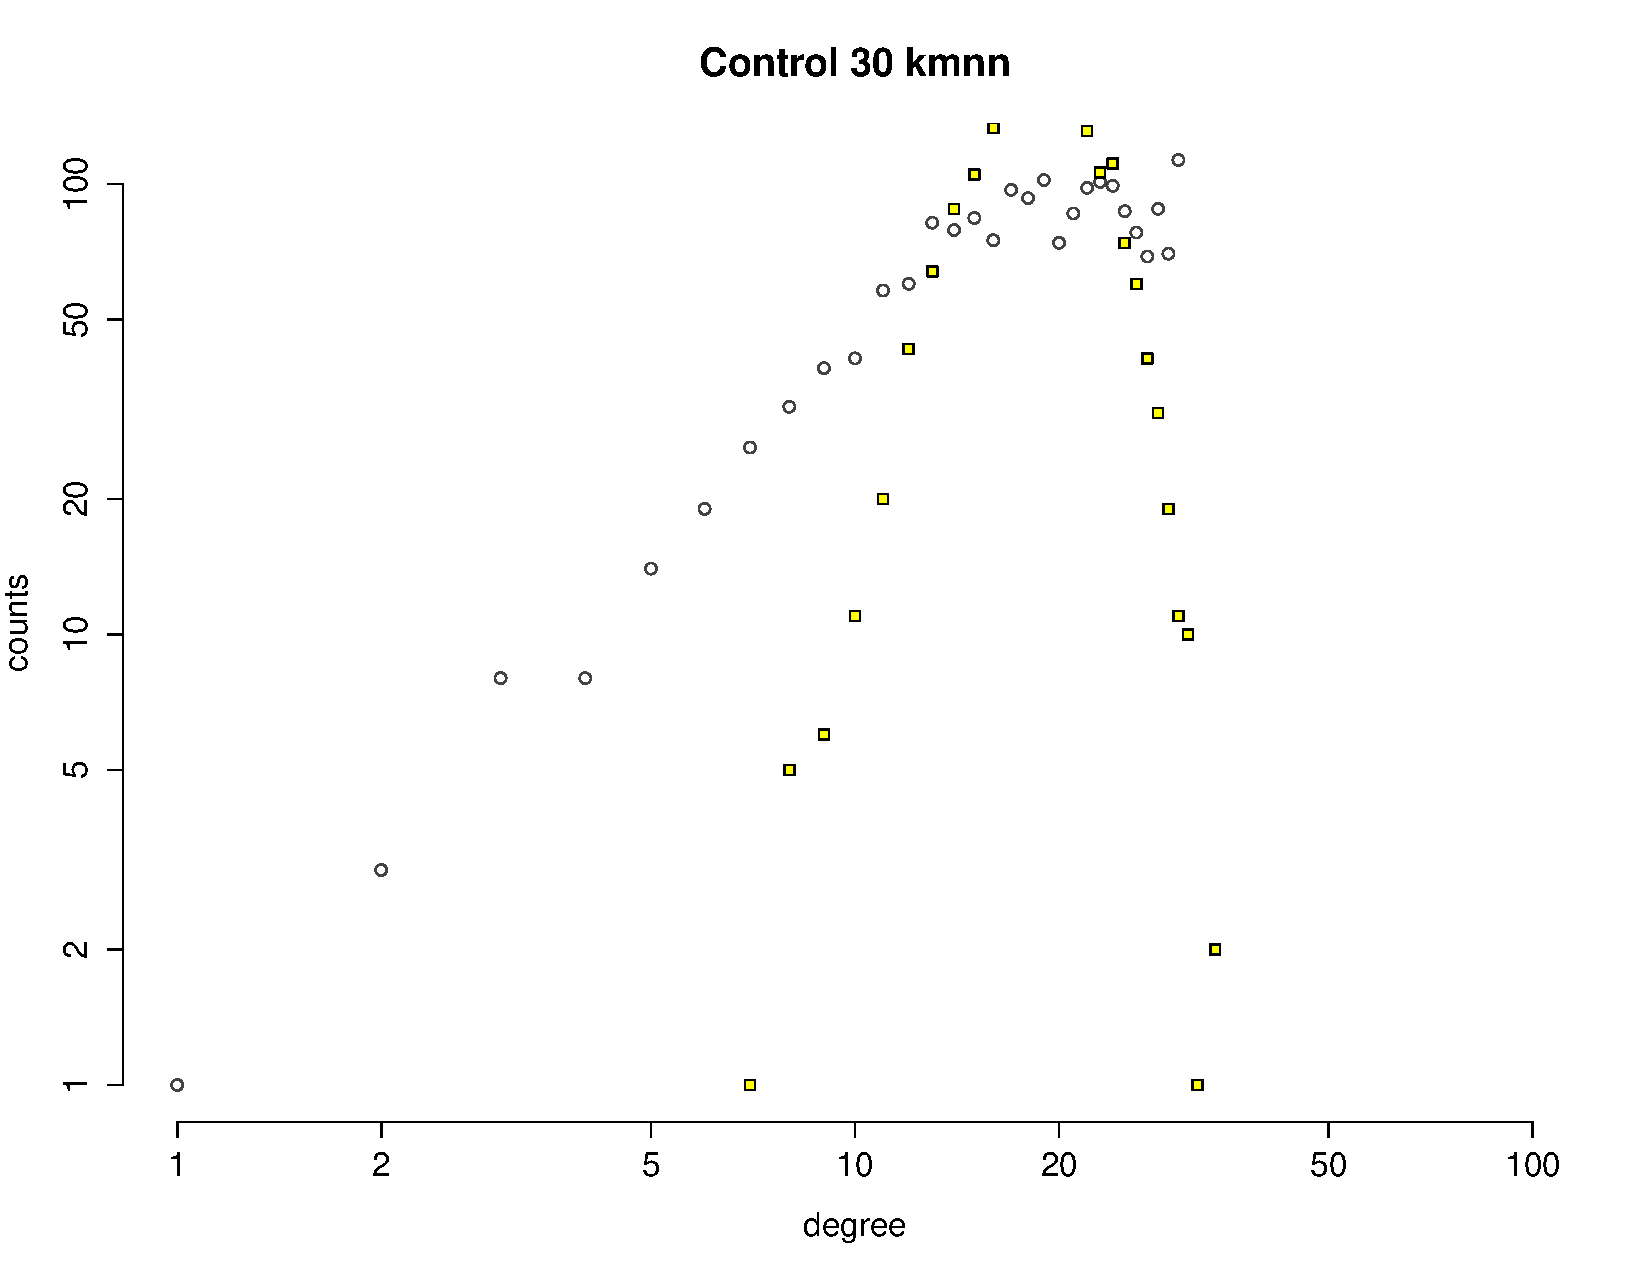
\includegraphics[width=1\textwidth]{erdos_renyi_vs_30kmnn.pdf}\\
%    Red y modelo nulo Erdös-Renyi
%    \column{0.5\textwidth}
%    \centering
%    Betweenness\\
%    \bigskip
%    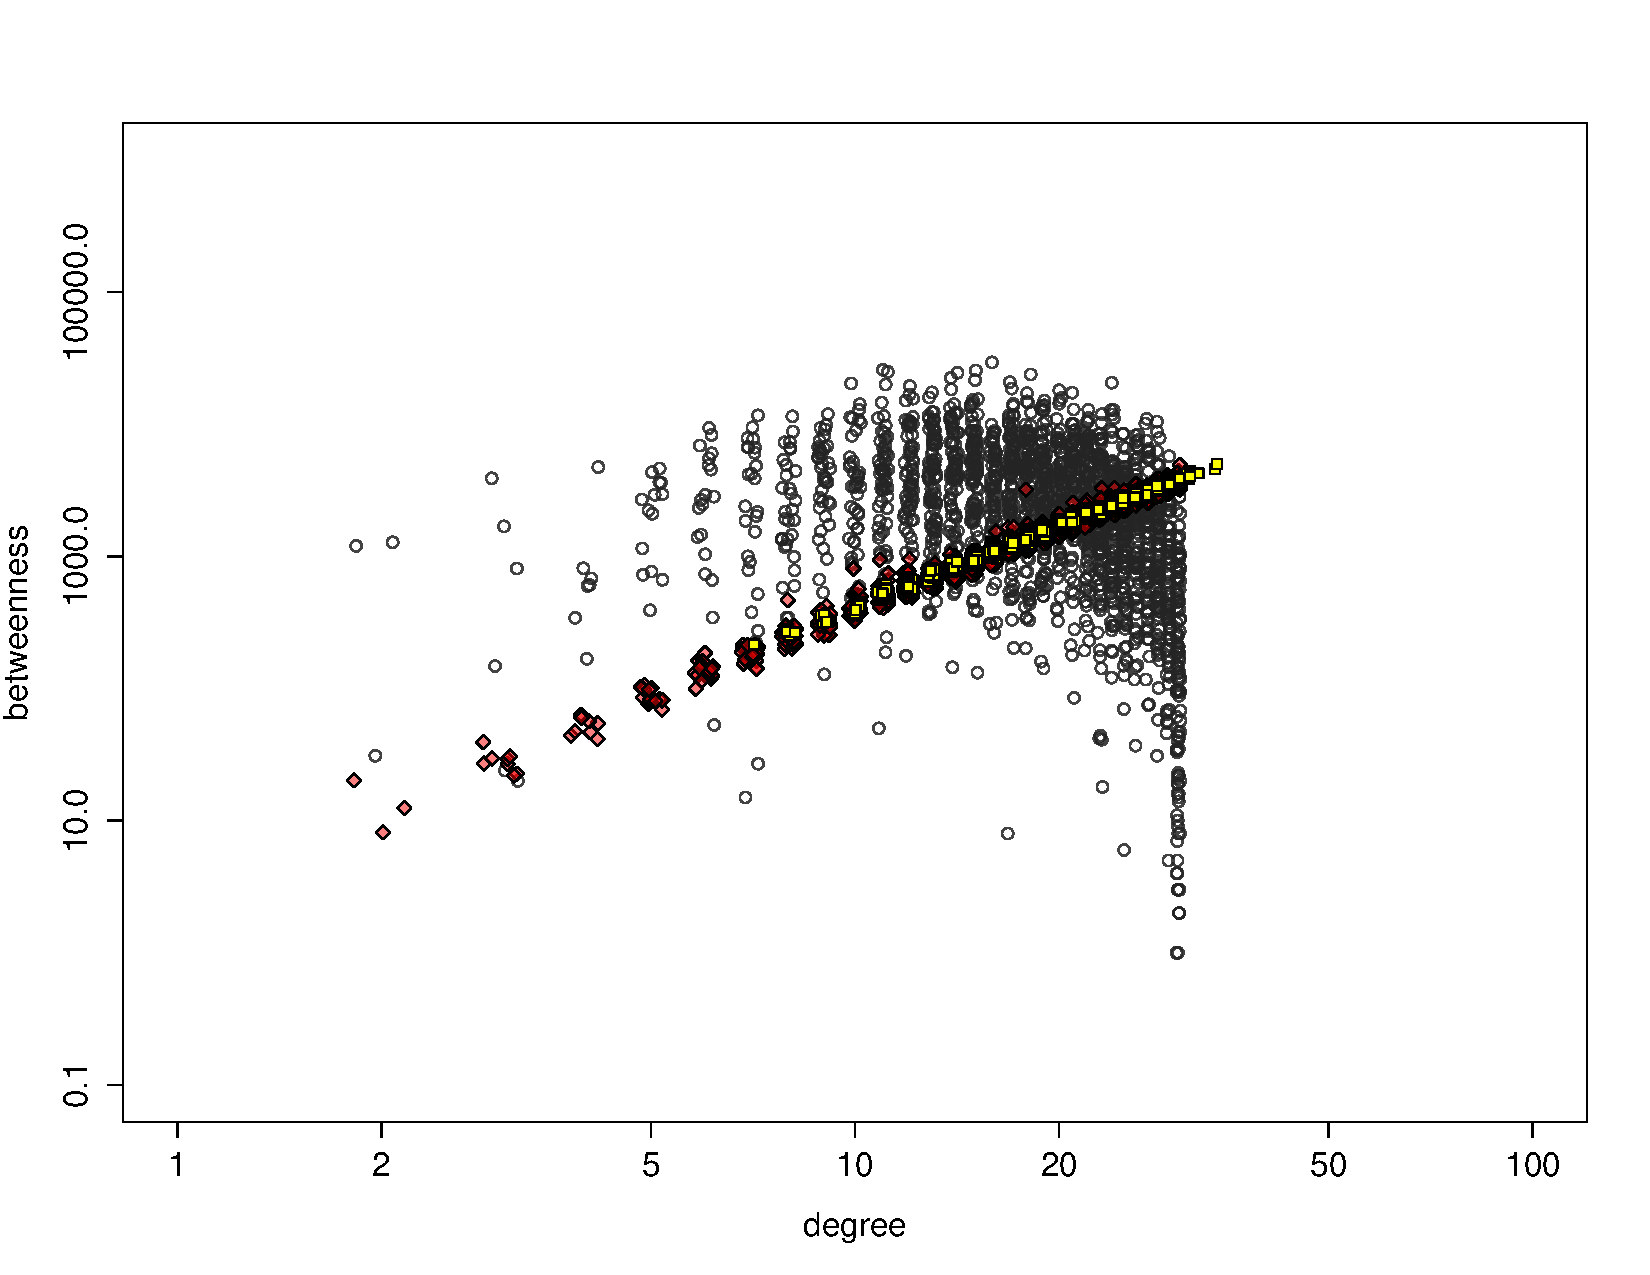
\includegraphics[width=1\textwidth]{betweenness_er_30_conf.pdf}\\
%    Red, modelo nulo Erdös-Renyi y modelo configuracional
%\end{columns}
%\end{frame}

\begin{frame}\frametitle{Red 30 primeros vecinos mutuos - vecindades locales} 
\centering
Queremos detectar zonas de alta coherencia.\\
\bigskip
\begin{columns}[T]
	\column{0.5\textwidth}
	 Generamos una red de 30 primeros vecinos mutuos y vamos a ver arista por arista, una localidad definida por los primeros vecinos:
	\bigskip
	\begin{itemize}
	\item $n_x$ nodos.
	\item $n_y$ nodos anotados.
	\item $wyn$ promedio de pesos de aristas en GO.
	\item $wyn_{anotados}$ promedio de pesos de aristas en GO con nodos anotados.	
	\end{itemize}
    \column{0.5\textwidth}
    \centering
    \bigskip
    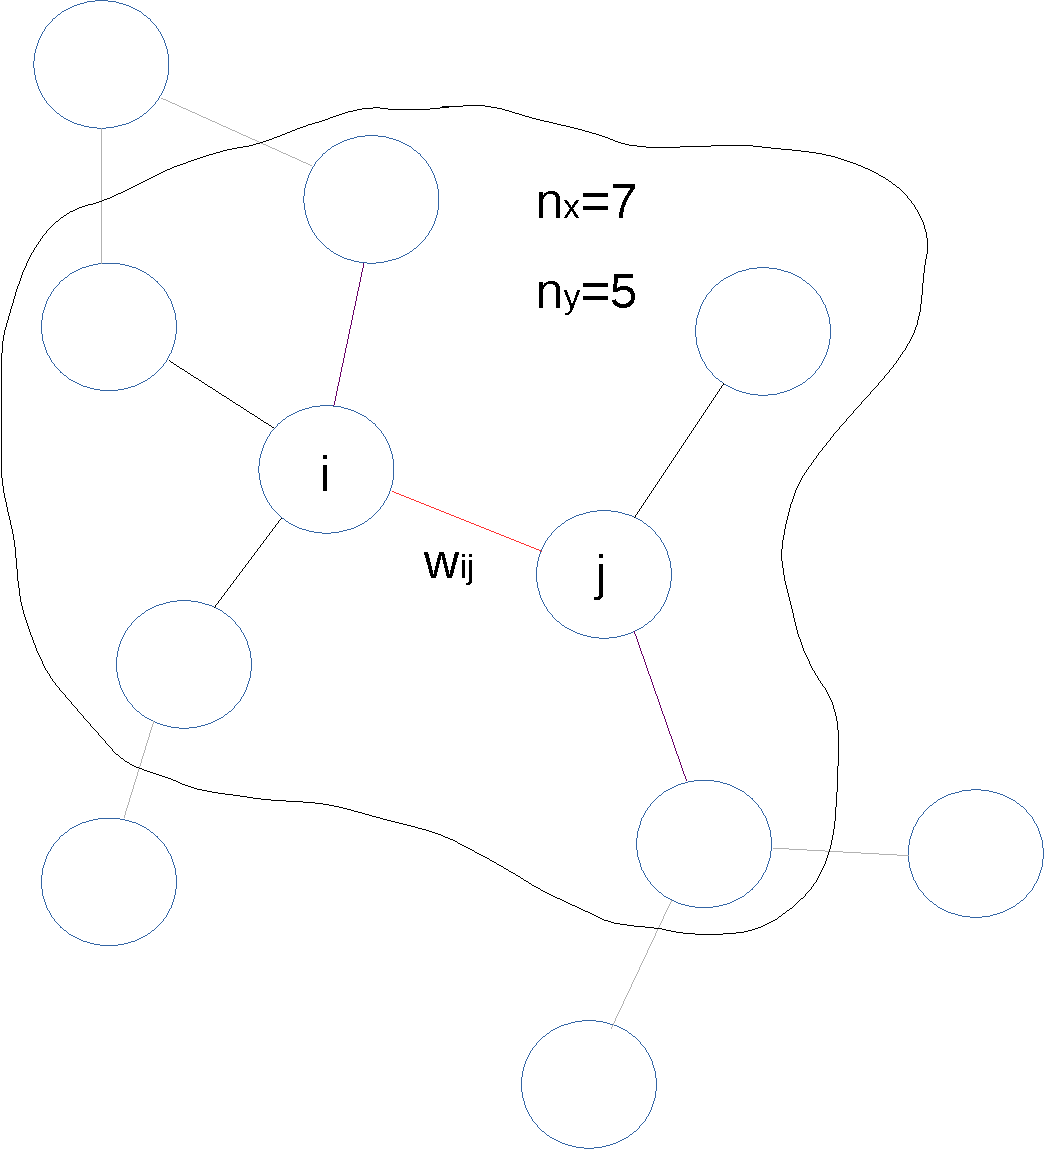
\includegraphics[width=0.8\textwidth]{vecindario_local.pdf}\\
    \bigskip
    \Fontvi
	A modo de ejemplo, la red para tratamiento ``Frío'' consta de 1951 nodos y 18436 aristas.
\end{columns}
\end{frame}

\begin{frame}\frametitle{Caracterización de vecindades locales tratamiento ``Frío''} 
\begin{columns}[T]
	\column{0.5\textwidth}
    \centering
    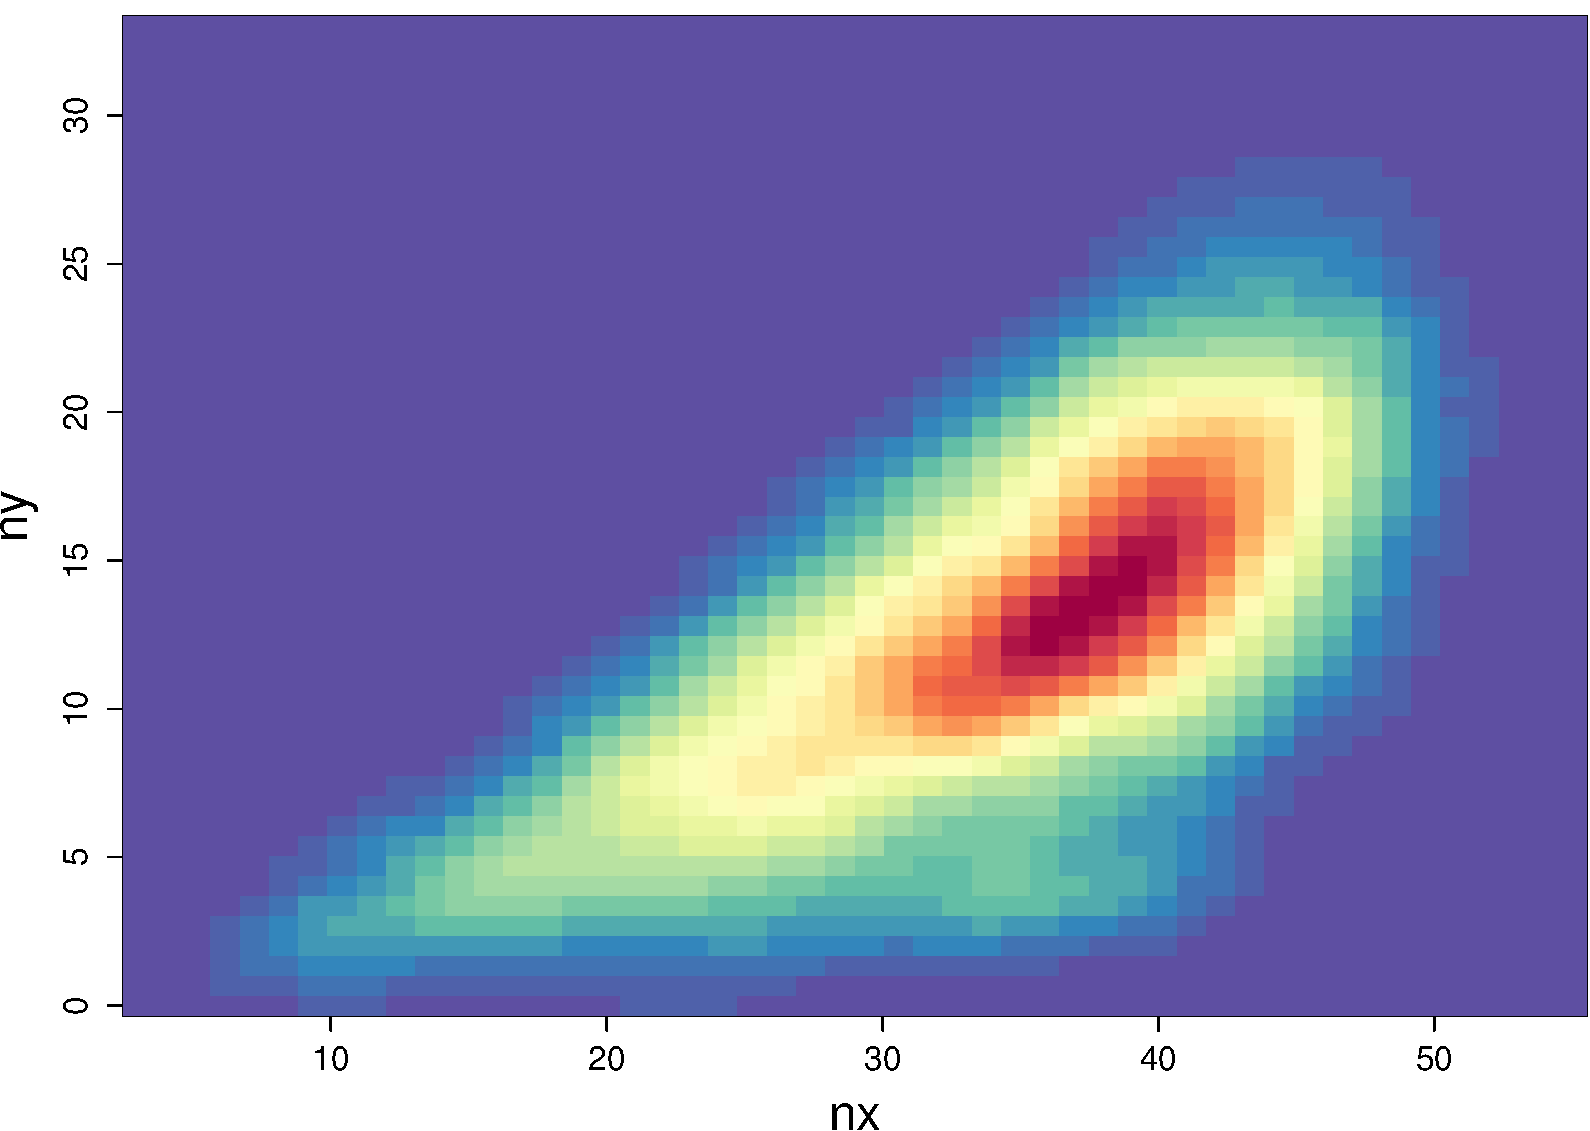
\includegraphics[width=0.90\textwidth]{nx_vs_ny.pdf}
    
    \centering
    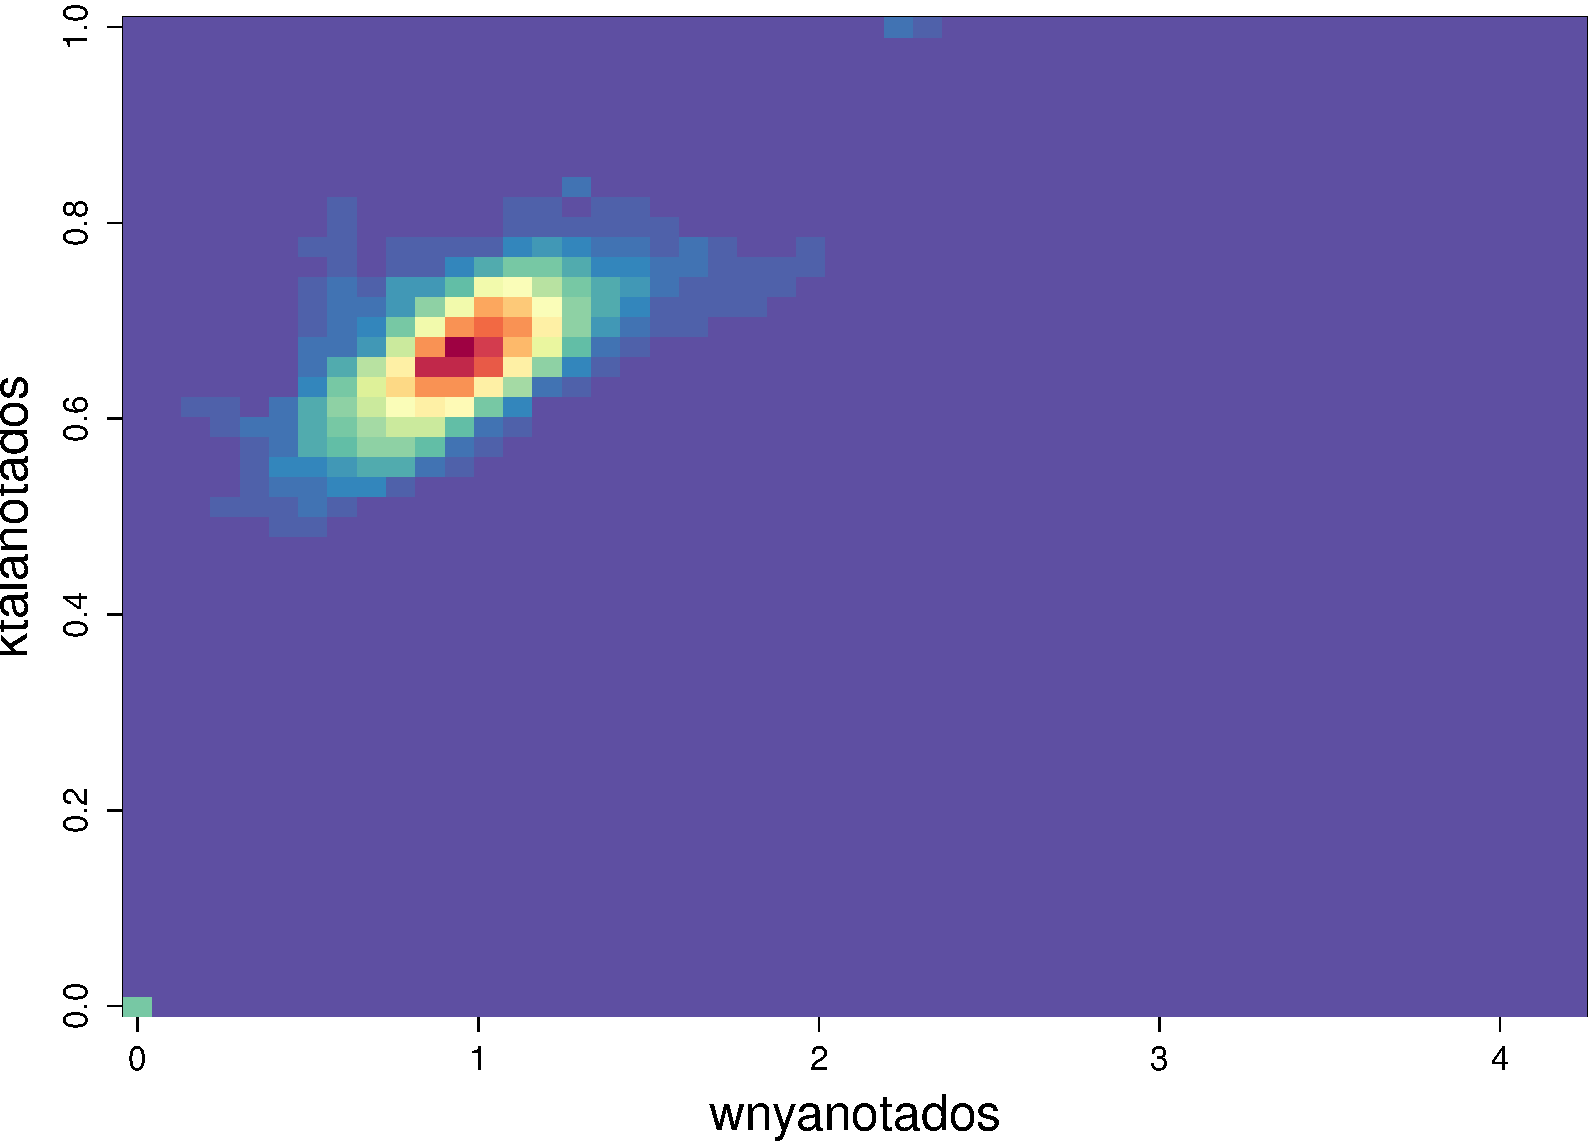
\includegraphics[width=0.90\textwidth]{lktaanotados_vs_wnyanotados.pdf}
	\column{0.5\textwidth}    
    \centering
    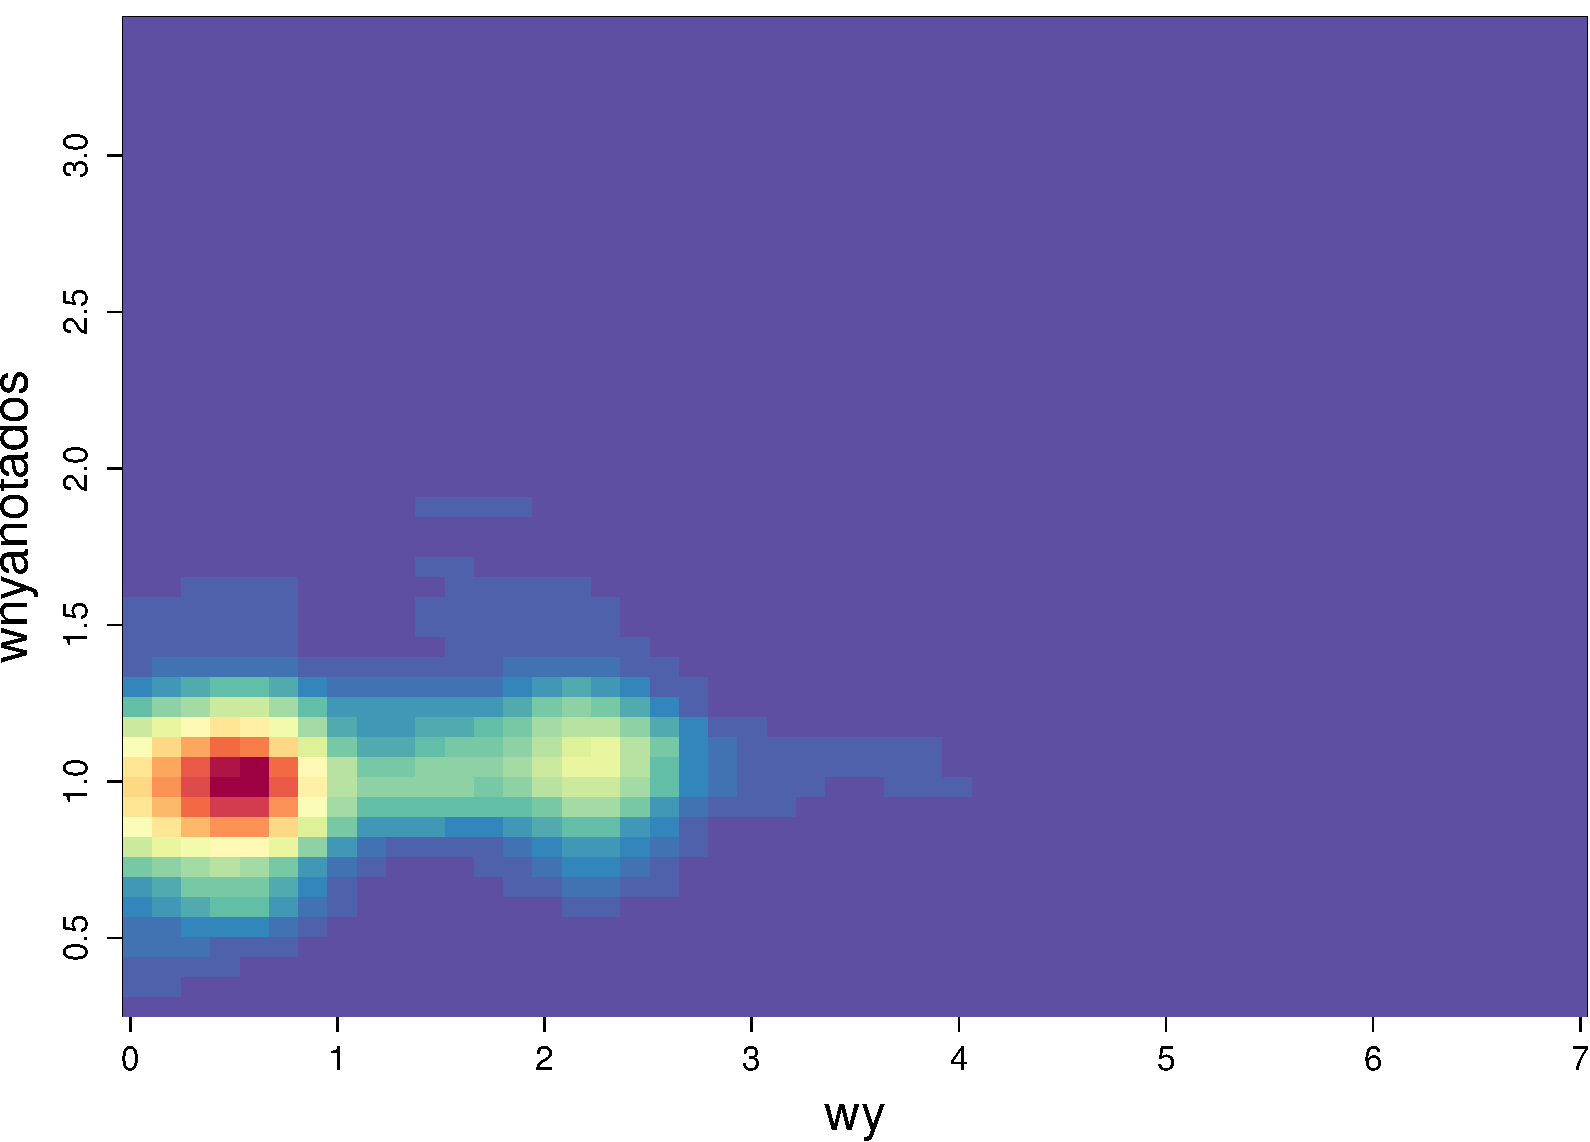
\includegraphics[width=0.90\textwidth]{wy_vs_wynanotados.pdf}
    
    \centering    
    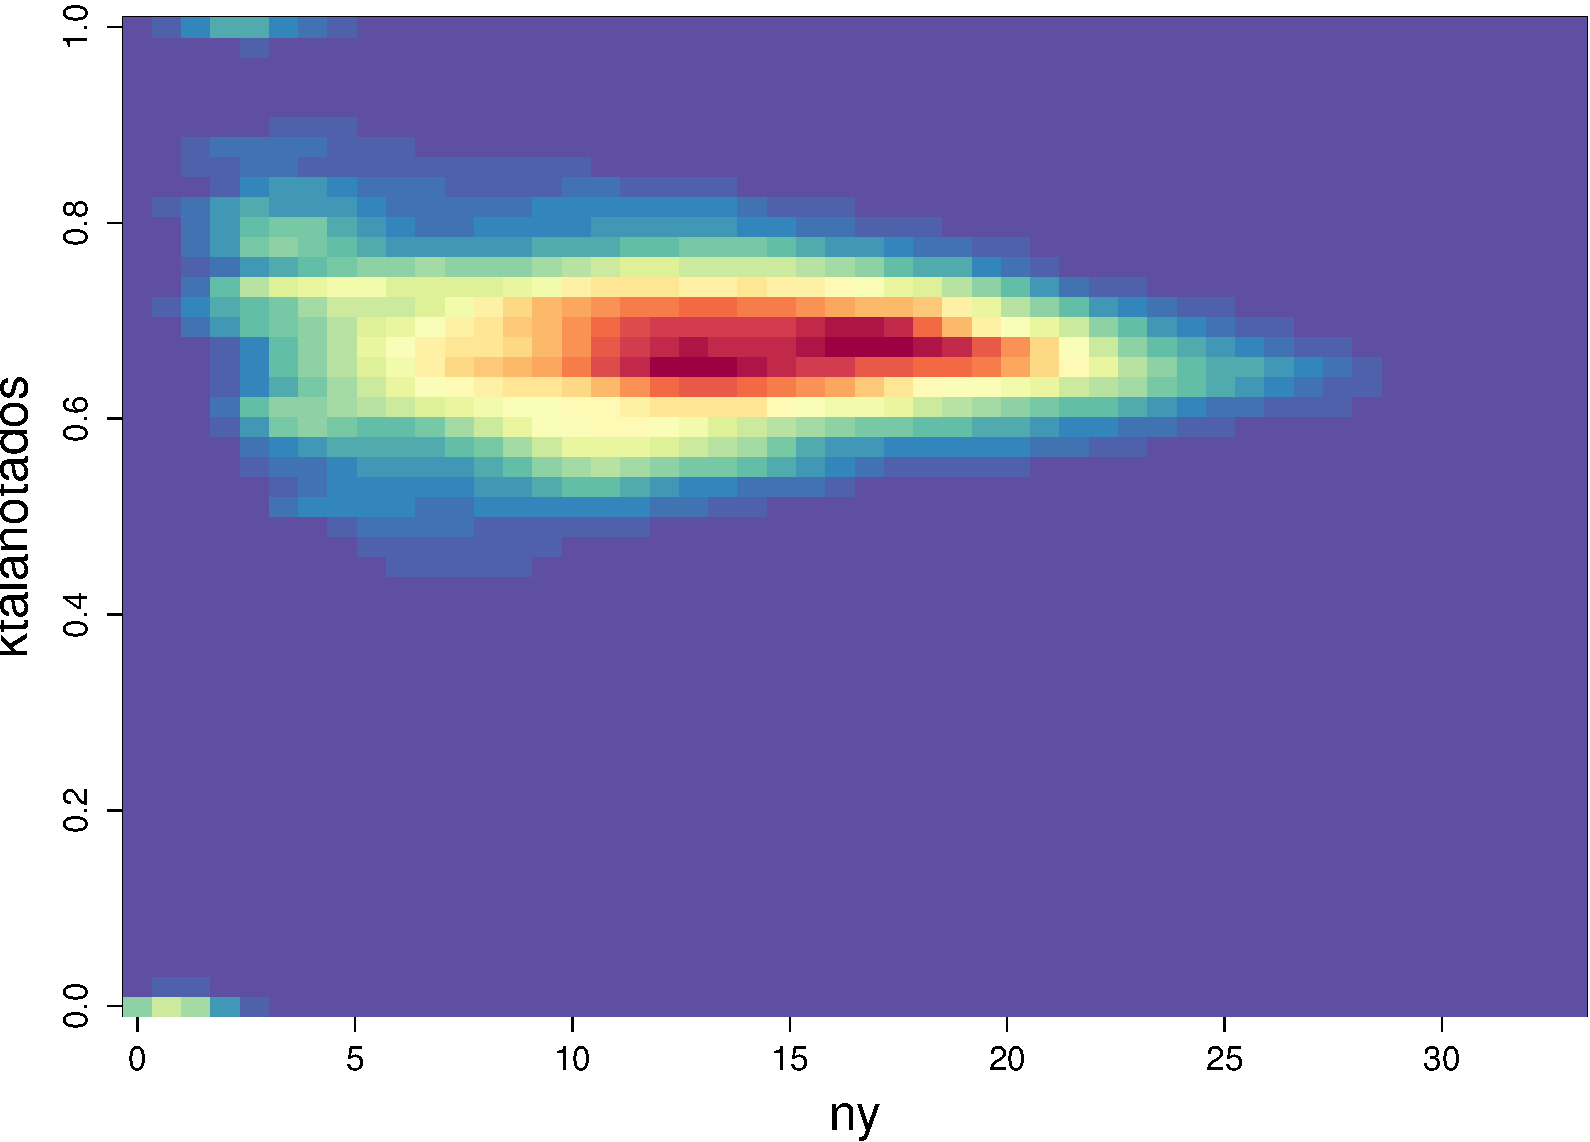
\includegraphics[width=0.90\textwidth]{lktaanotados_vs_nyanotados.pdf}
\end{columns}
\end{frame}

\subsubsection*{Métrica mixta}
\begin{frame}\frametitle{Métrica mixta} 
Dada una arista, el peso de una arista y el promedio de pesos, tenemos una manera de decir cuando una vecindad es o no biologicamente coherente.\\
\bigskip
Vamos a usar esto para encontrar grupos transcripcionales teniendo en cuenta las coherencias biológicas locales modificando los pesos:
\bigskip
\begin{equation}
	w_{ij} = simcor_{ij}^{\beta*stress_{ij}}
\end{equation}
Donde:
\begin{equation}
	stress_{ij} = \frac{KTA_{fondo}}{KTAl_{ij}}
\end{equation}
\bigskip
Típicamente el $stress$ oscila entre $0.8$ y $1.2$.\\
\bigskip
$\beta$ es un parámetro que permite aumentar aún más la homogeneidad de la red.
\end{frame}

\subsubsection*{Métodos heurísticos}

\begin{frame}\frametitle{Métodos heurísticos} 
\centering
Buscamos subestructura en los grupos a partir de la métrica mixta
\centering
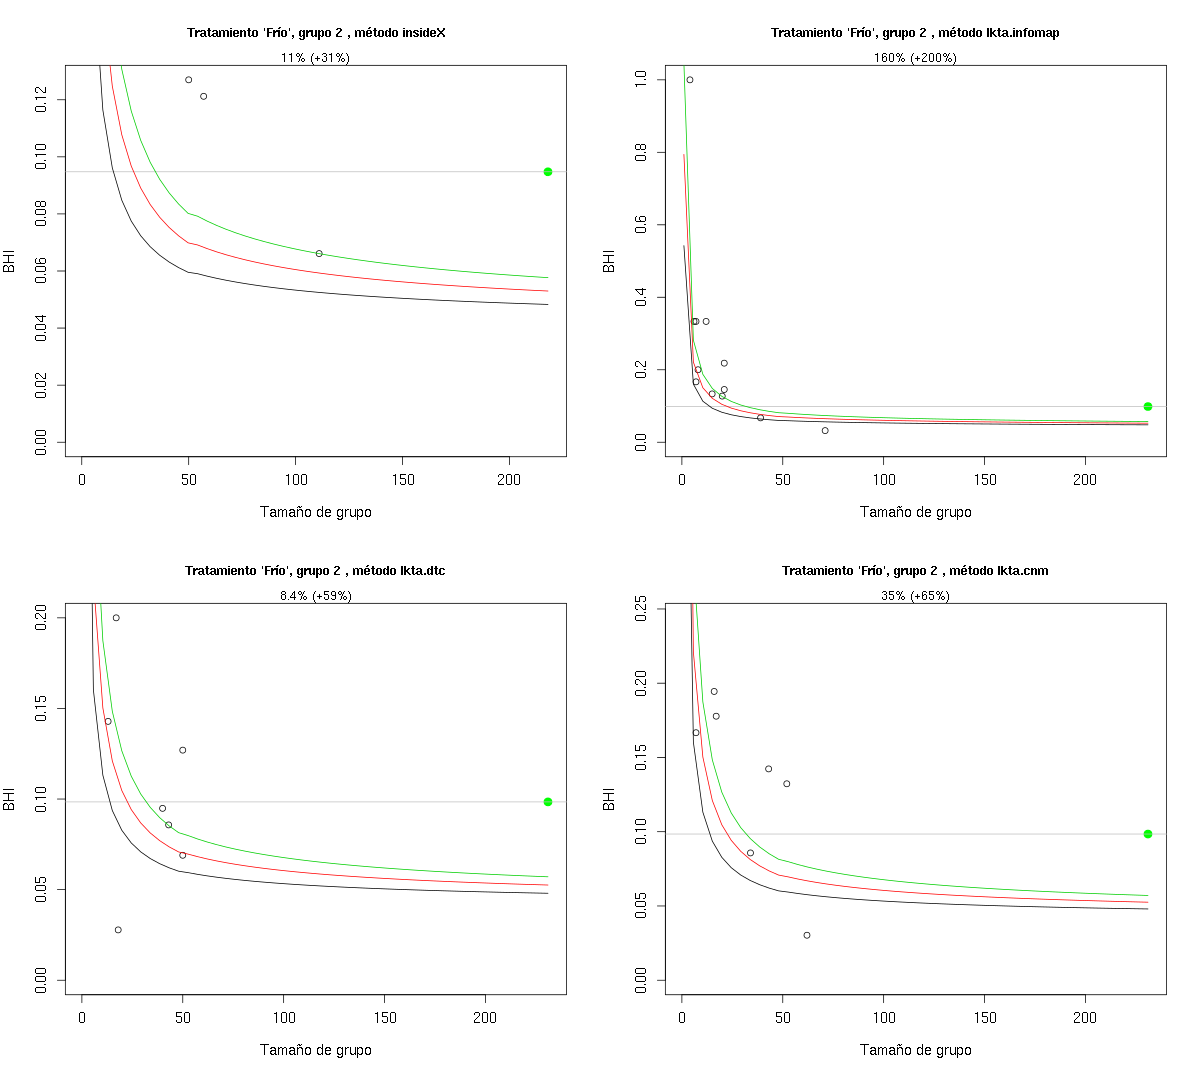
\includegraphics[width=0.7\textwidth]{metodos_mixtos_grupo_2.png}
\end{frame}

\begin{frame}\frametitle{Métodos heurísticos - caracterización de particiones} 
\centering
Caracterizamos los nuevos subgrupos hallados
\centering
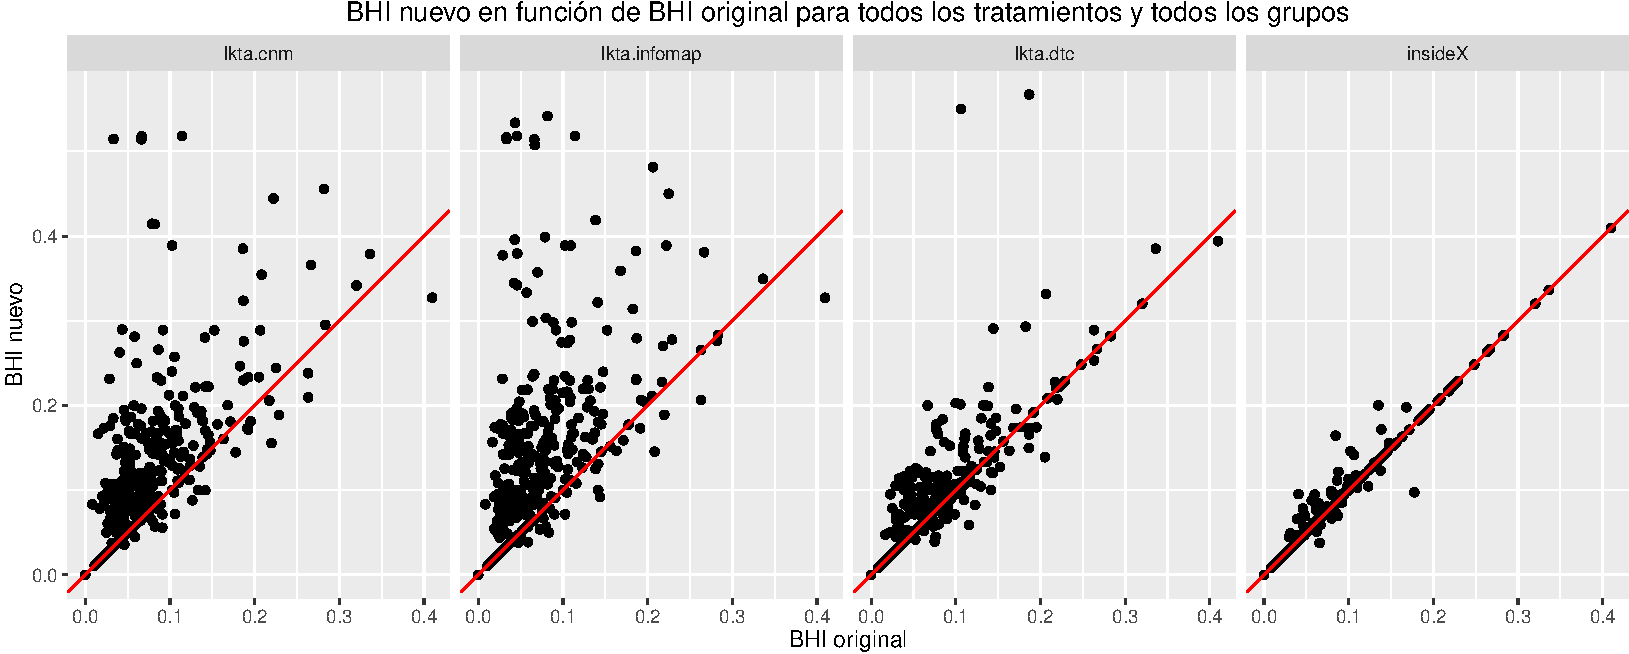
\includegraphics[width=1\textwidth]{bhi_nuevo_vs_bhi_original.pdf}
\end{frame}

\subsubsection*{Interpretación biológica}
\begin{frame}\frametitle{Interpretación biológica} 
\centering
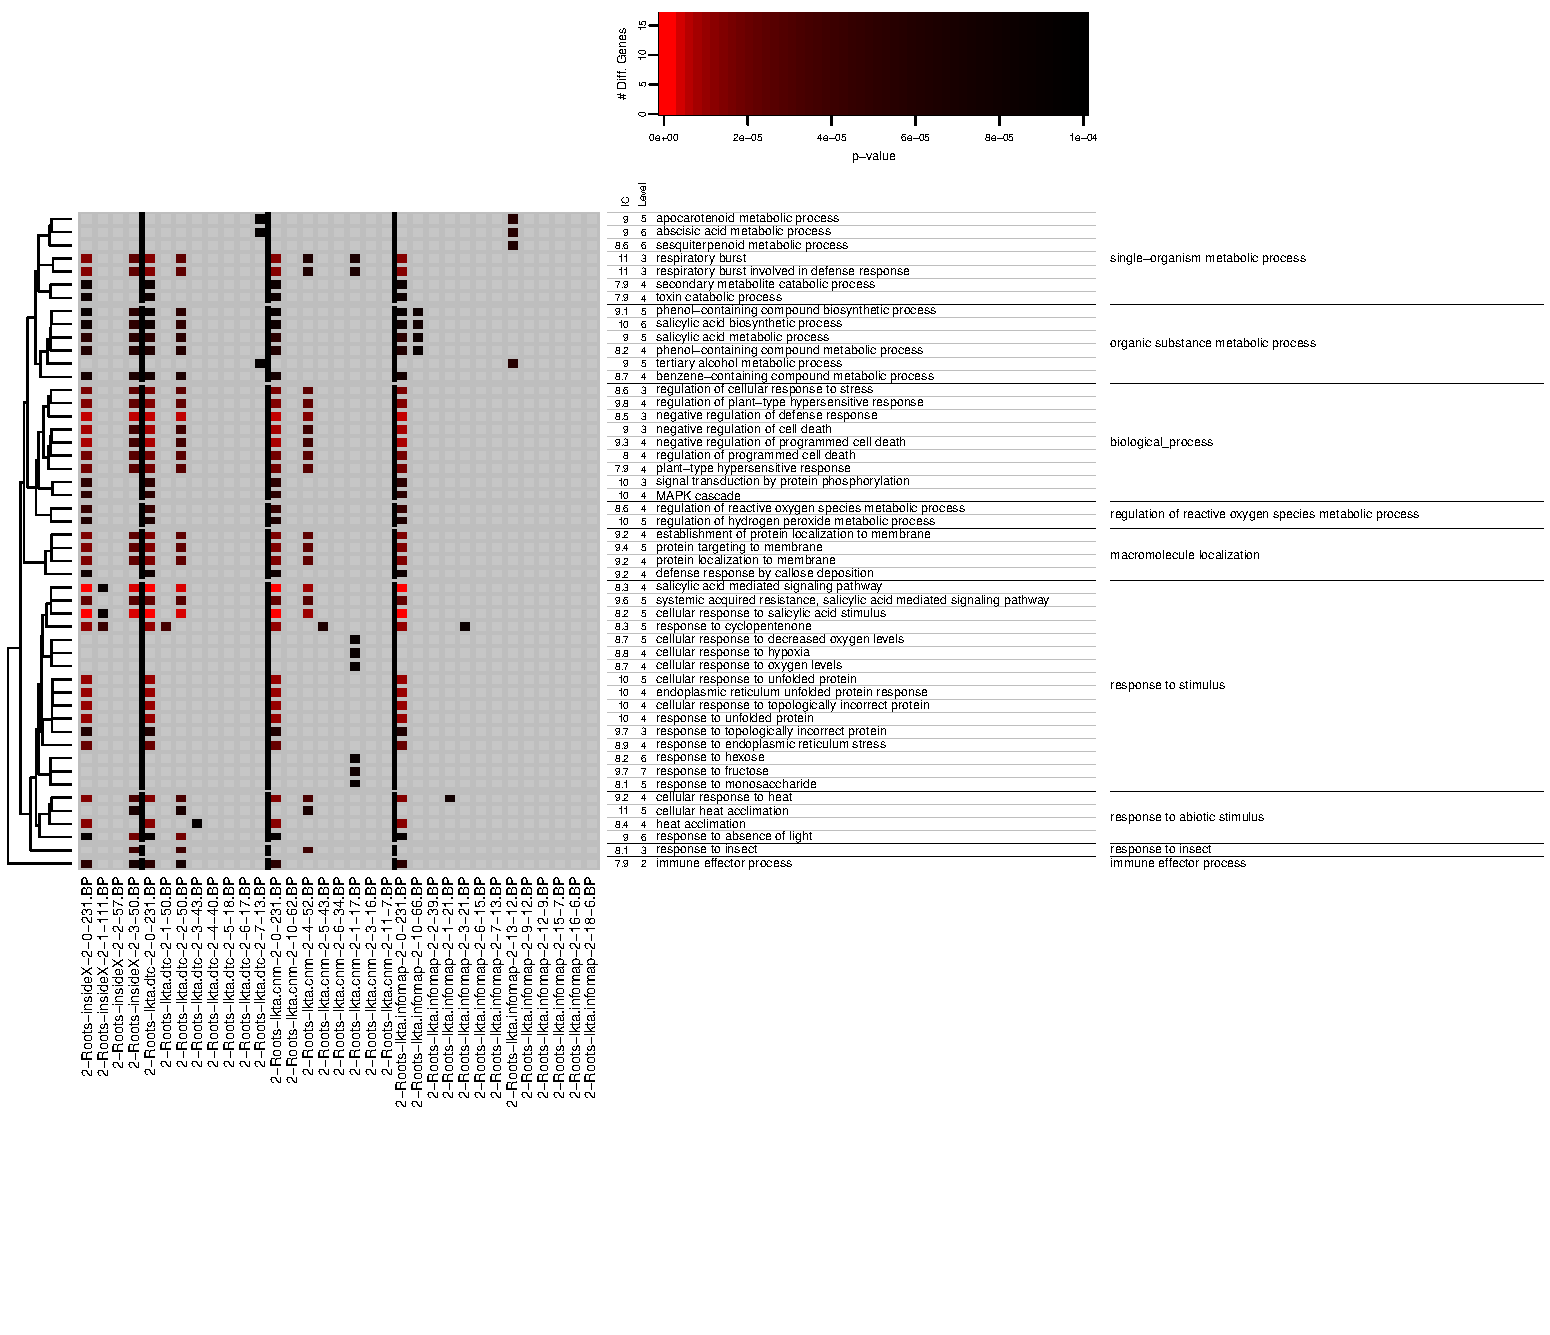
\includegraphics[width=0.9\textwidth]{fisher_grupo_2.pdf}
\end{frame}

\section{Conclusiones y perspectivas}
\begin{frame}\frametitle{Conclusiones y perspectivas}
\begin{itemize}
\item Mediante técnicas de agrupamiento de datos fue posible encontrar grupos de genes con perfiles de expresión altamente correlacionados.
\item Distintos métodos darán distintas particiones en función de la resolución que logran.
\item Mediante una métrica mixta fue posible encontrar particiones con alta homogeneidad biológica y con alta correlación transcripcional.
\item Utilizamos la ontología GO para dar una interpretación biológica a los grupos obtenidos y encontramos que en general, la granularidad óptima de los grupos fue de $\approx$ 50 genes.
\item Estas técnicas podrían funcionar como punto de partida para inferir funciones biológicas de genes de los que se tiene poco conocimiento.
\item Sería interesante en un futuro agregar la información contenida en otros espacios de conocimiento biológico, como ser vías metabólicas o redes de interacción de proteínas.
\end{itemize}
\end{frame}

\begin{frame}\frametitle{Agradecimientos}
\Large
\centering
¡Muchas gracias!\\
FOTO DEL GRUPO
%\includegraphics[width=0.9\textwidth]{}
\end{frame}

\end{document}